\setchapterpreamble[u]{\margintoc}
\chapter{Managing Input Data}
\label{chapter:input}

\epigraph{One home run is much better than two doubles.}{Steve Jobs}
\section{Introduction}

While advances in long-context language models\index{Long-context language models} (LCs) \cite{lee2024longcontextlanguagemodelssubsume} have expanded the amount of information these LLMs can process, significant challenges remain in managing and effectively utilizing extended data inputs:

\begin{itemize}
    \item LLMs are sensitive to input formatting and structure, requiring careful data preparation to achieve optimal results \cite{he2024doespromptformattingimpact, liu2024enhancingllmscognitionstructurization, tan2024htmlraghtmlbetterplain}.
    \item LLMs operate with knowledge cutoffs, providing potentially outdated information that may not reflect current reality and demonstrate problems with temporal knowledge accuracy \cite{amayuelas-etal-2024-knowledge}.
    \item LLMs exhibit drawbacks when processing long context facing ``lost-in-the-middle'' problems \cite{wu2024longdocumentsummaryevaluation} and struggle with less common but important information showing a systematic loss of long-tail knowledge \cite{kotha2024understanding}.
\end{itemize}

Motivated by these challenges, this chapter explores two key input data components:

\begin{enumerate}
    \item Data Pre-Processing: Parsing and chunking documents into a unified format that is suitable and manageable for LLMs to process effectively.
    \item Retrieval Augmentation: Augmenting LLMs with the ability to retrieve relevant, recent, and specialized information.
\end{enumerate}

In data parsing, we will explore some useful open source tools such as Docling and MarkItDown that help transform data into LLM-compatible formats, demonstrating their impact through a case study of structured information extraction from complex PDFs. In a second case study, we will introduce some chunking strategies to help LLMs process long inputs and implement a particular technique called Chunking with Contextual Linking the enables contextually relevant chunk processing.

In retrieval augmentation, we will explore how to enhance LLMs with semantic search capabilities for incorporating external context using RAGs~\sidenote{Meta AI first coined the term RAG in 2020 as a method to update LLM's world knowledge using a retrieval system: \url{https://arxiv.org/abs/2005.11401}} (Retrieval Augmented Generation) with Vector Databases such as ChromaDB. We also discuss whether RAGs will be really needed in the future given the rise of long-context language models.

While RAGs are useful for incorporating external context, they are not a silver bullet nor a mandatory component for all LLM applications. In our last case study, we demonstrate how long-context windows can be used to extract insights from a large knowledge base without the need for complex retrieval systems. We build a quiz generator from open books from Project Gutenberg. We will also explore some additional relevant techniques such as prompt caching and response verification through citations using ``Corpus-in-Context'' (CIC) Prompting \sidecite{lee2024longcontextlanguagemodelssubsume}.

By the chapter's conclusion, readers will possess relevant knowledge of input data management strategies for LLMs and practical expertise in selecting and implementing appropriate approaches and tools for specific use cases.
\section{Parsing Documents}
\label{parsing}

Data parsing and formatting play a critical role in LLMs performance \sidecite{he2024doespromptformattingimpact, liu2024enhancingllmscognitionstructurization, tan2024htmlraghtmlbetterplain}. Hence, building robust data ingestion and preprocessing pipelines is essential for any LLM application.

This section explores open source tools that streamline input data processing, in particular for parsing purposes, providing a unified interface for converting diverse data formats into standardized representations that LLMs can effectively process. By abstracting away format-specific complexities, they allow developers to focus on core application logic rather than parsing implementation details while maximizing LLM's performance.

We will cover open source tools that provide parsing capabilities for a wide range of data formats. And we will show how some of these tools can be used to extract structured information from complex PDFs demonstrating how the quality of the parser can impact LLM's performance.

\subsection{MarkItDown}

MarkItDown\index{MarkItDown} \sidecite{microsoft2024markitdown} is a Python package and CLI tool developed by the Microsoft for converting various file formats to Markdown. It supports a wide range of formats including PDF, PowerPoint, Word, Excel, images (with OCR and EXIF metadata), audio (with transcription), HTML, and other text-based formats making it a useful tool for document indexing and LLM-based applications.

Key features:
\begin{marginlisting}[-1.35cm]
	\caption{MarkItDown Sample Usage.}
    \label{lst:markitdown}
	\vspace{0.6cm}
	\begin{lstlisting}[language=Python,style=kaolstplain]
from markitdown import MarkItDown

md = MarkItDown()
result = md.convert("doc.pdf")
print(result.text_content)
	\end{lstlisting}
\end{marginlisting}
\begin{itemize}
    \item Simple command-line and Python API interfaces
    \item Support for multiple file formats
    \item Optional LLM integration for enhanced image descriptions
    \item Batch processing capabilities
    \item Docker support for containerized usage
\end{itemize}

\subsection{Docling}

Docling\index{Docling} \sidecite{docling2024github} is a Python package developed by IBM Research for parsing and converting documents into various formats. It provides advanced document understanding capabilities with a focus on maintaining document structure and formatting.

Key features:
\begin{marginlisting}[-1.35cm]
	\caption{Docling Sample Usage.}
    \label{lst:docling}
	\vspace{0.6cm}
	\begin{lstlisting}[language=Python,style=kaolstplain]
from docling.document_converter import DocumentConverter

converter = DocumentConverter()
result = converter.convert("doc.pdf")
print(result.document.export_to_markdown())
	\end{lstlisting}
\end{marginlisting}
\begin{itemize}
    \item Support for multiple document formats (PDF, DOCX, PPTX, XLSX, Images, HTML, etc.)
    \item Advanced PDF parsing including layout analysis and table extraction 
    \item Unified document representation format
    \item Integration with LlamaIndex and LangChain
    \item OCR support for scanned documents
    \item Simple CLI interface
\end{itemize}

\subsection{Structured Data Extraction\index{Structured output}}

A common use case where document parsing matters is structured data extraction, particularly in the presence of complex formatting and layout. In this case study, we will extract the economic forecasts from Merrill Lynch's CIO Capital Market Outlook released on December 16, 2024 \sidecite{merrill2024}. We will focus on page 7 of this document, which contains several economic variables organized in a mix of tables, text and images (see Figure \ref{forecast}).

\begin{figure*}[h!]
\centering
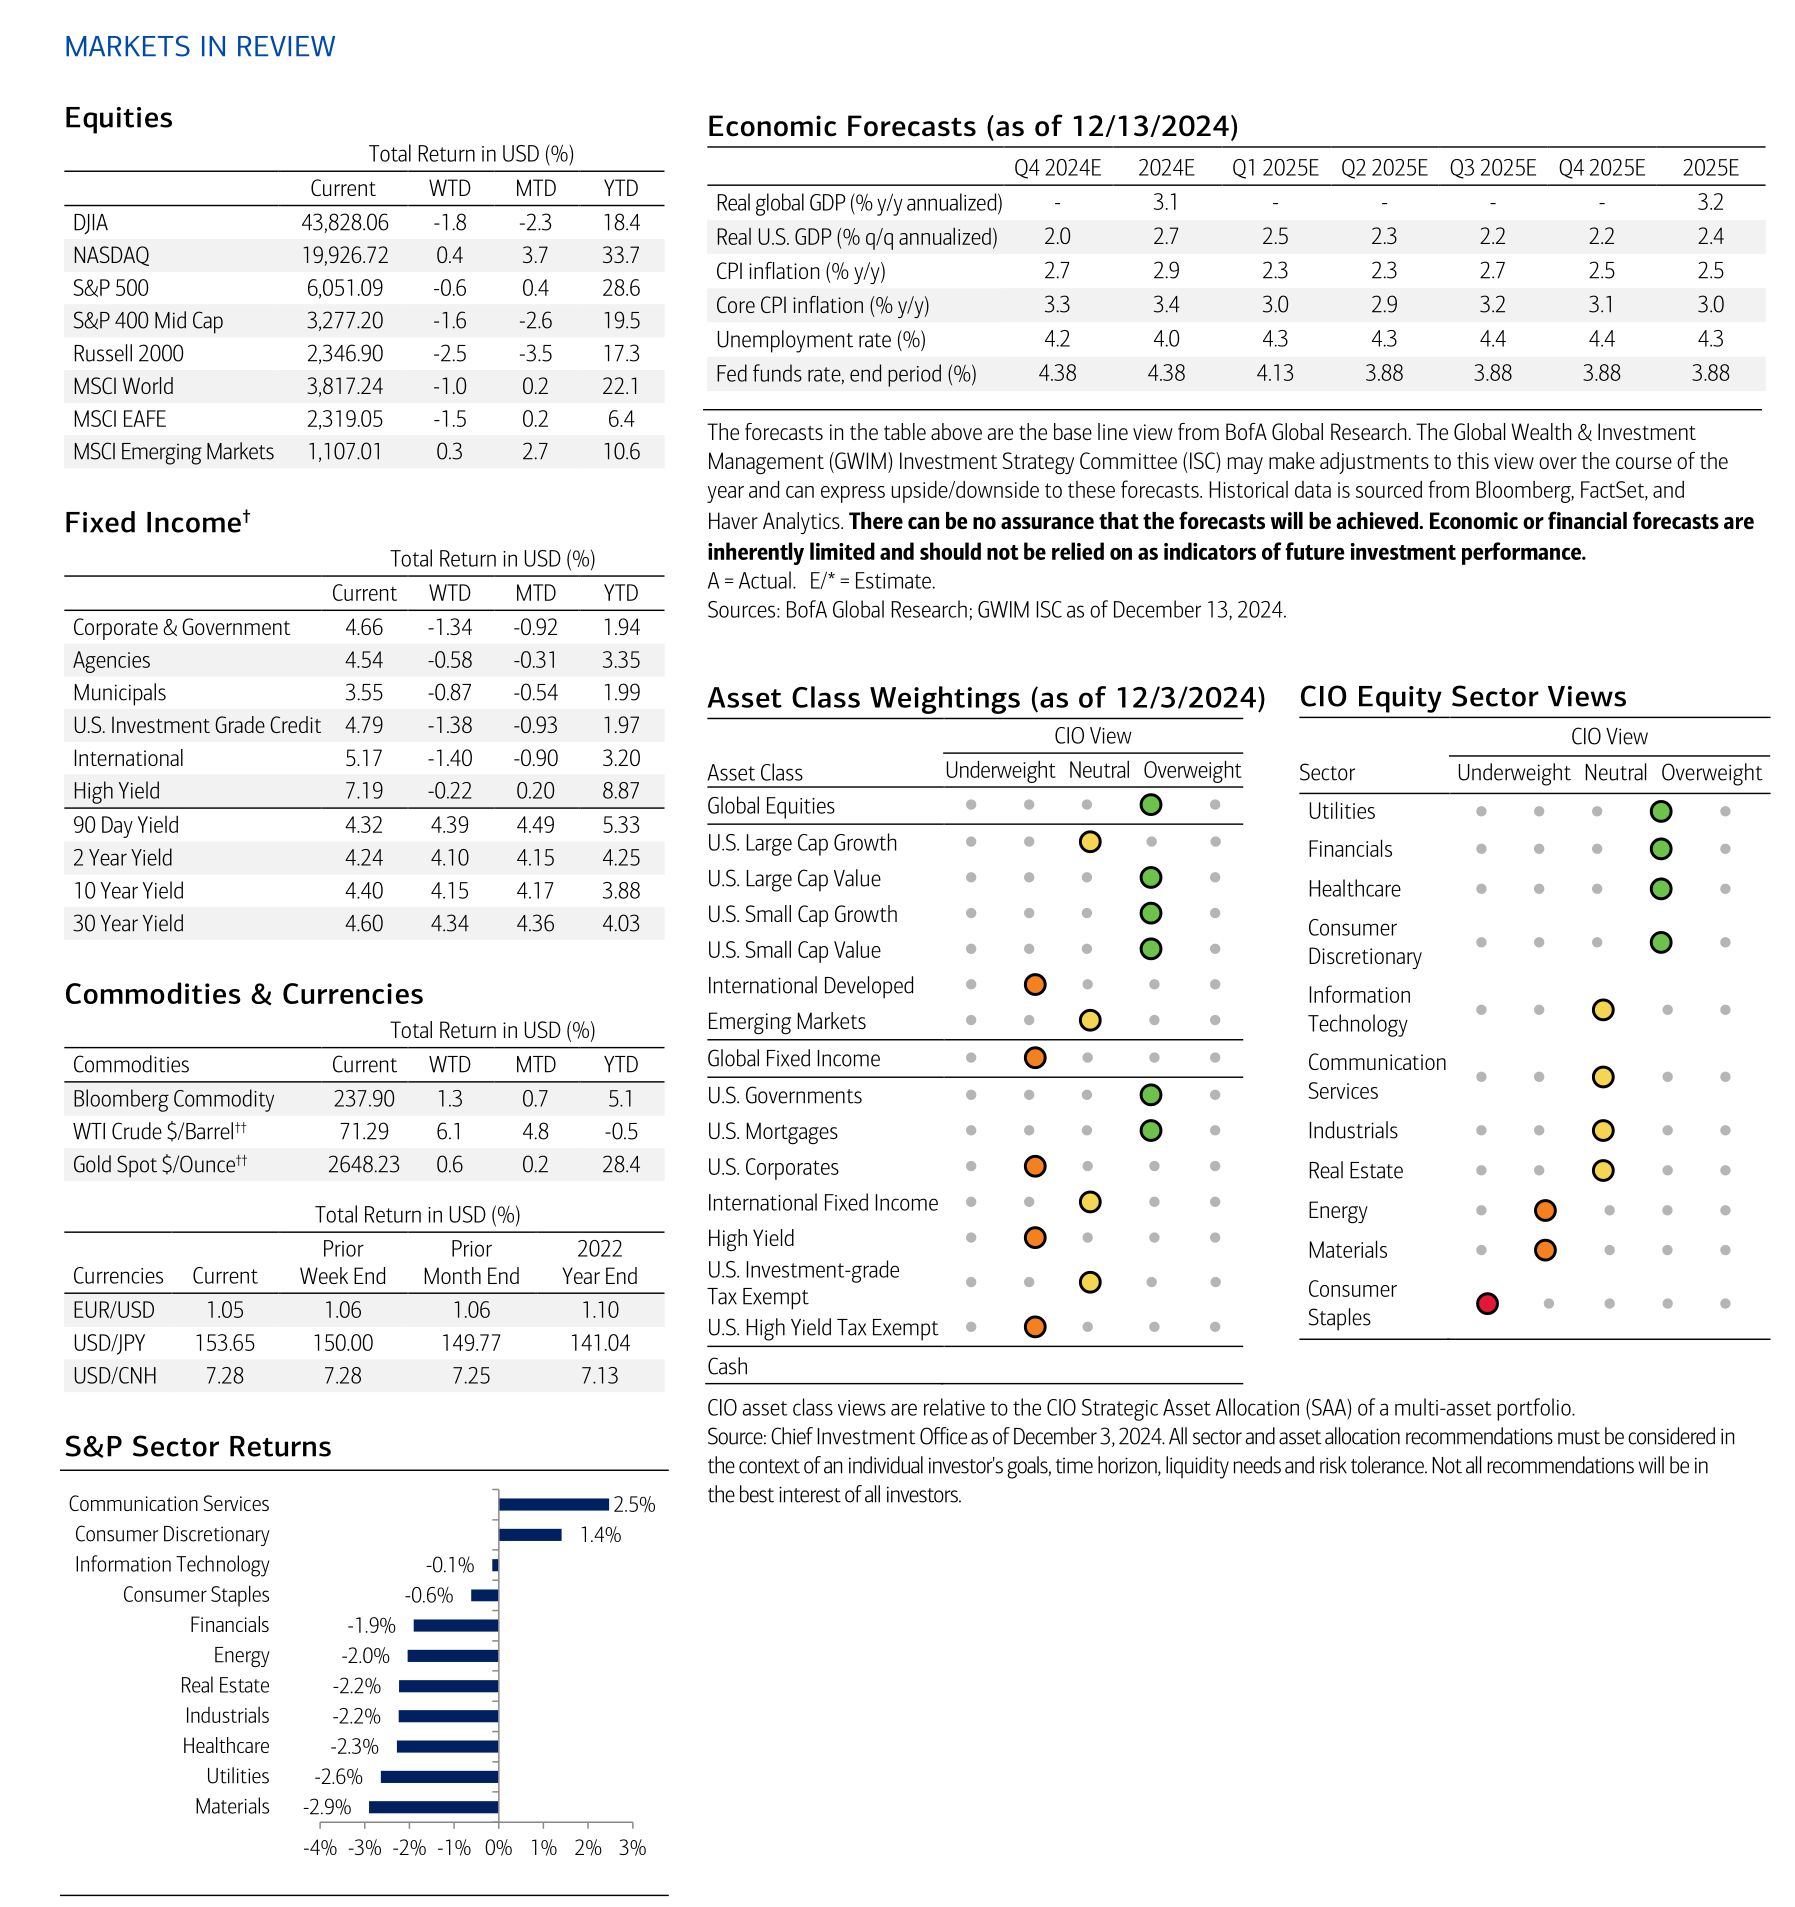
\includegraphics{input/forecast.png}
\caption{Merrill Lynch's CIO Capital Market Outlook released on December 16, 2024 \cite{merrill2024}}
\label{forecast}
\end{figure*}

\begin{minted}{python}
FORECAST_FILE_PATH = "../data/input/forecast.pdf"
\end{minted}

First, we will use MarkItDown to extract the text content from the document.

\begin{minted}{python}
from markitdown import MarkItDown

md = MarkItDown()
forecast_result_md = md.convert(FORECAST_FILE_PATH).text_content
\end{minted}

Next, we will do the same with Docling.

\begin{minted}{python}
from docling.document_converter import DocumentConverter

converter = DocumentConverter()
forecast_result_docling = converter.convert(source).document.export_to_markdown()
\end{minted}
How similar are the two results? We can use use Levenshtein distance\index{Levenshtein distance}~\sidecite{10.5555/1822502} to measure the similarity between the two results. We will also calculate a naive score using the \texttt{SequenceMatcher} from the \texttt{difflib} package, which is a simple measure of similarity between two strings based on the number of matches in the longest common subsequence.

\begin{minted}{python}
import Levenshtein
def levenshtein_similarity(text1: str, text2: str) -> float:
    """
    Calculate normalized Levenshtein distance
    Returns value between 0 (completely different) and 1 (identical)
    """
    distance = Levenshtein.distance(text1, text2)
    max_len = max(len(text1), len(text2))
    return 1 - (distance / max_len)

from difflib import SequenceMatcher
def simple_similarity(text1: str, text2: str) -> float:
    """
    Calculate similarity ratio using SequenceMatcher
    Returns value between 0 (completely different) and 1 (identical)
    """
    return SequenceMatcher(None, text1, text2).ratio()
\end{minted}

\begin{minted}{python}
levenshtein_similarity(forecast_result_md, forecast_result_docling)
\end{minted}

Levenshtein similarity score:
\begin{verbatim}
0.13985705461925346
\end{verbatim}


\begin{minted}{python}
simple_similarity(forecast_result_md, forecast_result_docling)
\end{minted}

\texttt{SequenceMatcher} similarity score: 
\begin{verbatim}
0.17779960707269155
\end{verbatim}


The results show significant differences between the two approaches, with similarity scores of approximately 13.98\% and 17.77\% for Levenshtein and \texttt{SequenceMatcher}, respectively.

Docling produces a well-structured markdown output that clearly displays the economic variables and their forecasts. In contrast, MarkItDown's output, while containing the same information, lacks structure and readability. The implications of these differences will be explored in the following section.
%OK

\textbf{Docling's Result}

\begin{minted}{python}
display(Markdown(forecast_result_docling))
\end{minted}

\begin{figure}[H]
\centering
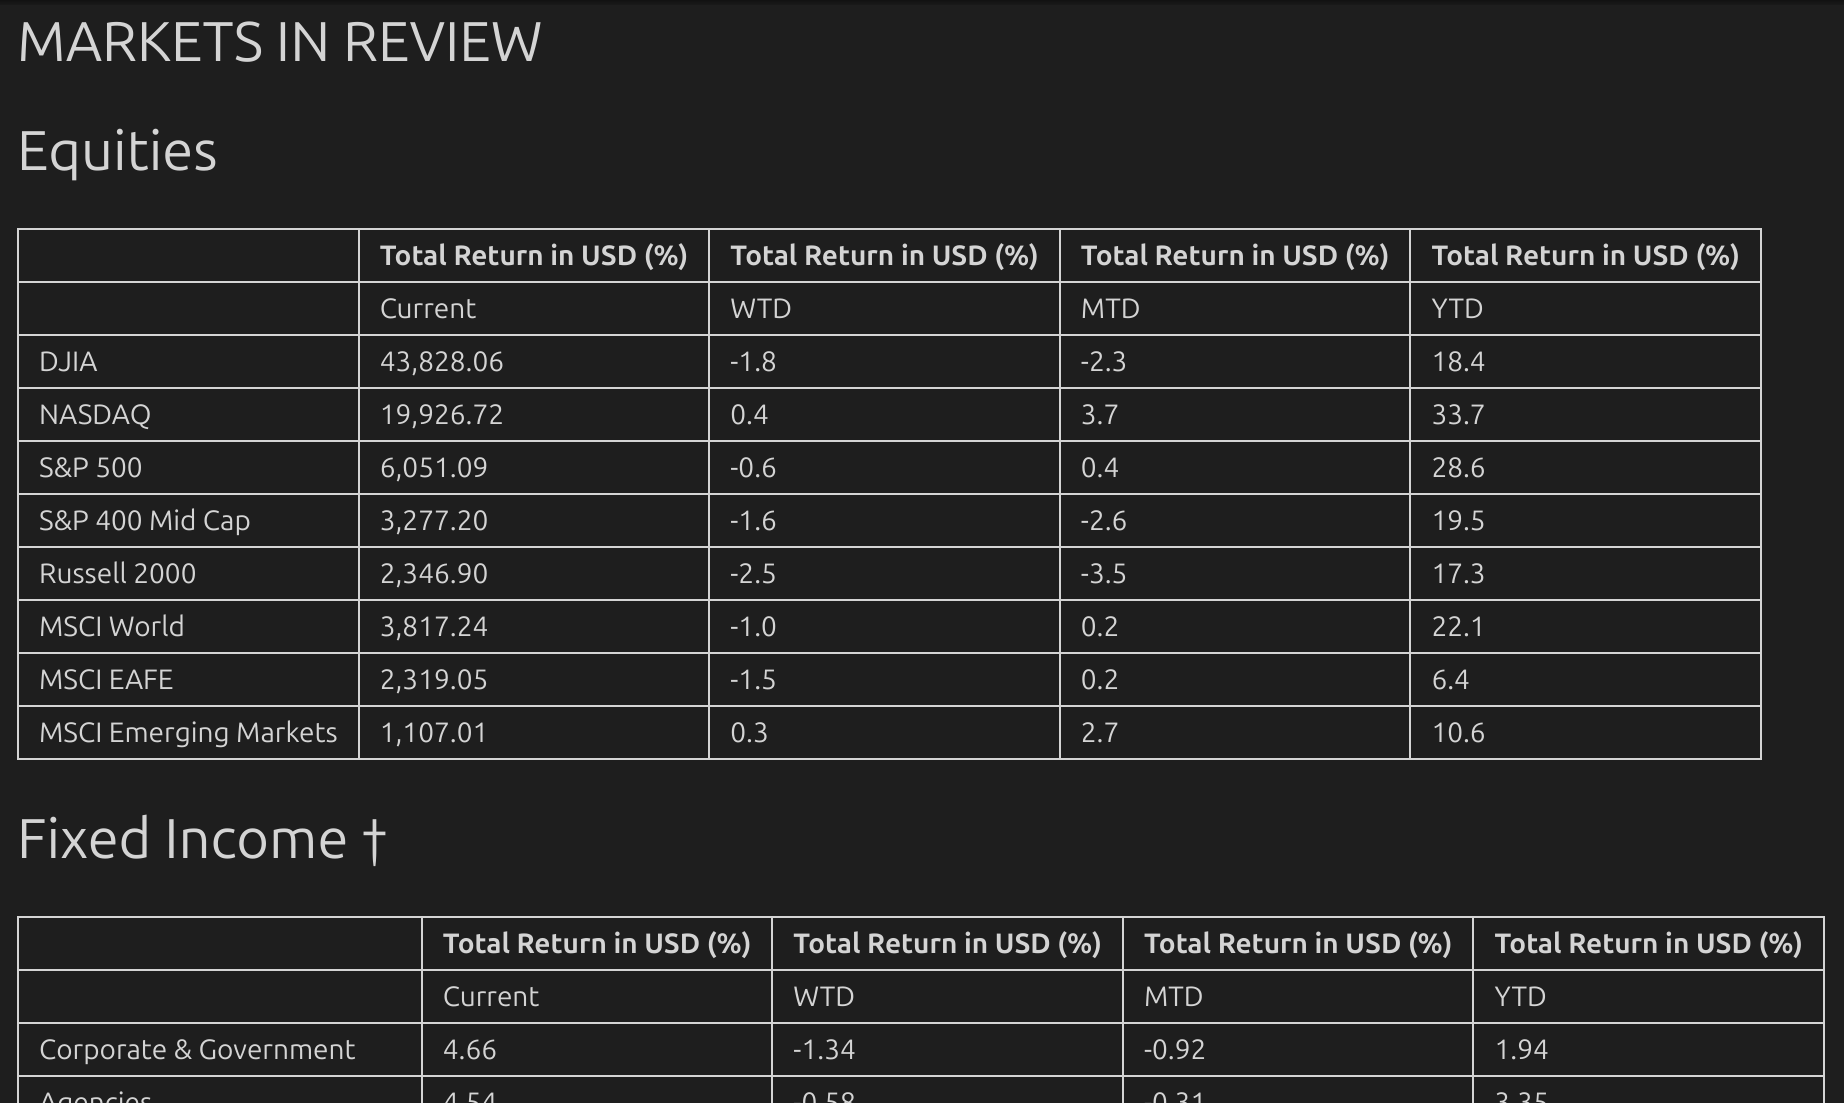
\includegraphics{input/docling.png}
\caption{An extract of Docling's parsed result.}
\label{docling}
\end{figure}

\textbf{MarkItDown's result}

\begin{minted}{python}
from IPython.display import display, Markdown
display(Markdown(forecast_result_md[:500]))
\end{minted}

{numref}`markitdown` shows part of the parsed result from MarkItDown.
\begin{figure}[H]
\centering
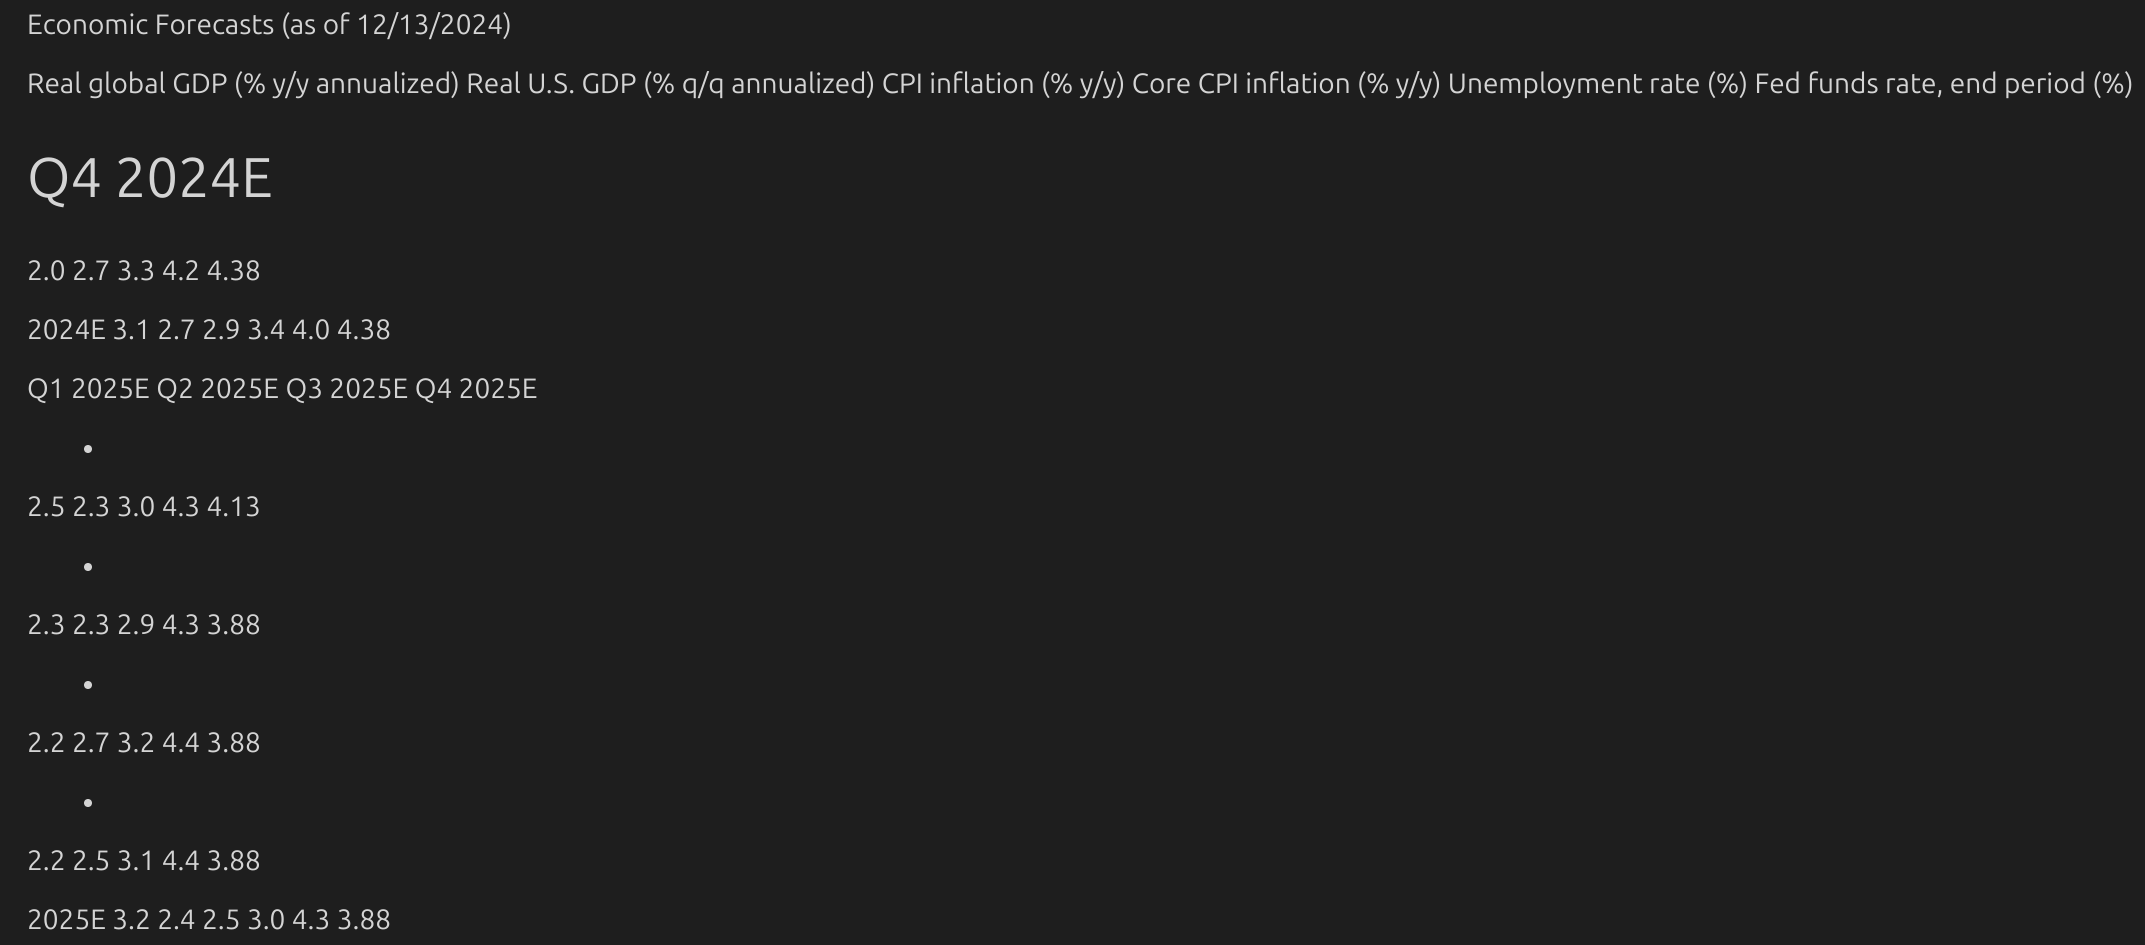
\includegraphics{input/markitdown.png}
\caption{An extract of MarkItDown's parsed result.}
\label{markitdown}
\end{figure}
Now, let's focus on the economic forecasts. In particular, we are interested in extracting the CIO's 2025E forecasts. This could be a useful predictive indicator for the economy in 2025.

\begin{figure}[H]
\centering
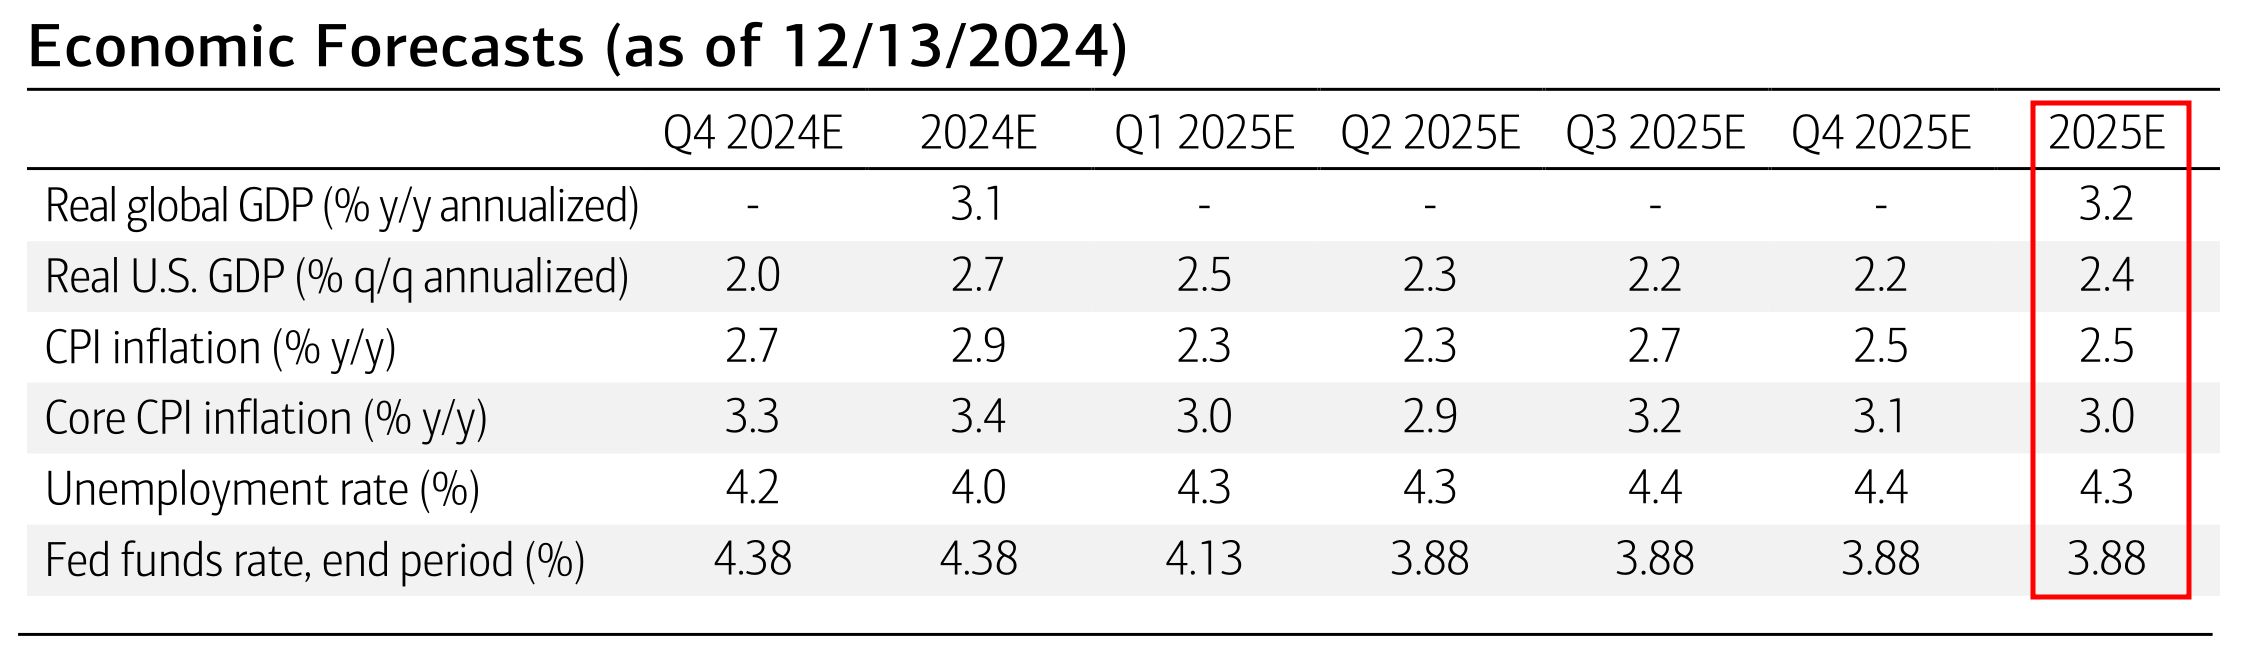
\includegraphics{input/2025.png}
\caption{Merrill Lynch's CIO Economic Forecasts.}
\label{forecast2025}
\end{figure}

We will define a \texttt{Forecast} pydantic\index{Pydantic} model to represent an economic forecast composed of a \texttt{financial\_variable} and a \texttt{financial\_forecast}. We will also define a \texttt{EconForecast} pydantic model to represent the list of economic forecasts we want to extract from the document.

\begin{minted}{python}
from pydantic import BaseModel
class Forecast(BaseModel):
    financial_variable: str
    financial_forecast: float
class EconForecast(BaseModel):
    forecasts: list[Forecast]
\end{minted}

We write a simple function to extract the economic forecasts from the document using an LLM model (with structured output) with the following prompt template, where \texttt{extract\_prompt} represents the kind of data the user would like to extract and \texttt{doc} is the input document.

\begin{minted}{python}
BASE_PROMPT = f"""
    ROLE: You are an expert at structured data extraction. 
    TASK: Extract the following data {extract_prompt} from input DOCUMENT
    FORMAT: The output should be a JSON object with 'financial_variable' as key and 'financial_forecast' as value.
    """
prompt = f"{BASE_PROMPT} \n\n DOCUMENT: {doc}"
\end{minted}

\begin{minted}{python}
def extract_from_doc(extract_prompt: str,  doc: str, client) -> EconForecast:

    BASE_PROMPT = f"""
    ROLE: You are an expert at structured data extraction. 
    TASK: Extract the following data {extract_prompt} from input DOCUMENT
    FORMAT: The output should be a JSON object with 'financial_variable' as key and 'financial_forecast' as value.
    """
    prompt = f"{BASE_PROMPT} \n\n DOCUMENT: {doc}"
    completion = client.beta.chat.completions.parse(
        model="gpt-4o-mini",
        messages=[
            {
                "role": "system",
                "content": prompt
            },
            {"role": "user", "content": doc}
        ],
        response_format=EconForecast
    )
    return completion.choices[0].message.parsed
\end{minted}
\begin{minted}{python}
from dotenv import load_dotenv
import os

# Load environment variables from .env file
load_dotenv(override=True)
from openai import OpenAI
client = OpenAI()
\end{minted}

The user then calls the \texttt{extract\_from\_doc} function simply defining that ``Economic Forecasts for 2025E'' is the data they would like to extract from the document. We perform the extraction twice, once with MarkItDown and once with Docling.

\begin{minted}{python}
extract_prompt = "Economic Forecasts for 2025E"
md_financials = extract_from_doc(extract_prompt, forecast_result_md, client)
docling_financials = extract_from_doc(extract_prompt, forecast_result_docling, client)
\end{minted}
The response is an \texttt{EconForecast} object containing a list of \texttt{Forecast} objects, as defined in the pydantic model. We can then convert the response to a pandas DataFrame for easier comparison.

\begin{minted}{python}
md_financials
\end{minted}


\begin{verbatim}
EconForecast(forecasts=[Forecast(financial_variable='Real global GDP (% y/y annualized)', financial_forecast=3.2), Forecast(financial_variable='Real U.S. GDP (% q/q annualized)', financial_forecast=2.4), Forecast(financial_variable='CPI inflation (% y/y)', financial_forecast=2.5), Forecast(financial_variable='Core CPI inflation (% y/y)', financial_forecast=3.0), Forecast(financial_variable='Unemployment rate (%)', financial_forecast=4.3), Forecast(financial_variable='Fed funds rate, end period (%)', financial_forecast=3.88)])
\end{verbatim}


\begin{minted}{python}
df_md_forecasts = pd.DataFrame([(f.financial_variable, f.financial_forecast) for f in md_financials.forecasts], 
                      columns=['Variable', 'Forecast'])
df_docling_forecasts = pd.DataFrame([(f.financial_variable, f.financial_forecast) for f in docling_forecasts.forecasts], 
                      columns=['Variable', 'Forecast'])

df_md_forecasts
\end{minted}



\begin{table}[h!]
\centering
\caption{Economic Forecasts for 2025E using MarkItDown Parser}
\begin{tabular}{lc}
\hline
\textbf{Variable} & \textbf{Forecast} \\
\hline
Real global GDP (\% y/y annualized) & 3.20 \\
Real U.S. GDP (\% q/q annualized) & 2.40 \\
CPI inflation (\% y/y) & 2.50 \\
Core CPI inflation (\% y/y) & 3.00 \\
Unemployment rate (\%) & 4.30 \\
Fed funds rate, end period (\%) & 3.88 \\
\hline
\end{tabular}
\label{tab:markitdown-forecasts}
\end{table}

\begin{minted}{python}
df_docling_forecasts
\end{minted}

\begin{table}[h!]
\centering
\caption{Economic Forecasts for 2025E using Docling Parser}
\begin{tabular}{lc}
\hline
\textbf{Variable} & \textbf{Forecast} \\
\hline
Real global GDP (\% y/y annualized) & 3.20 \\
Real U.S. GDP (\% q/q annualized) & 2.40 \\
CPI inflation (\% y/y) & 2.50 \\
Core CPI inflation (\% y/y) & 3.00 \\
Unemployment rate (\%) & 4.30 \\
Fed funds rate, end period (\%) & 3.88 \\
\hline
\end{tabular}
\label{tab:docling-forecasts}
\end{table}


The results from MarkItDown and Docling are identical and accurately match the true values from the document. This demonstrates that despite MarkItDown's output appearing less readable from a human perspective, both approaches enabled the LLM to successfully extract the economic forecast data with equal accuracy, in this particular case.

Next, let's focus on the asset class weightings. We will extract the asset class weightings from the document and compare the results from MarkItDown and Docling. The information is now presented in a quite different structure as we can see in Figure \ref{fig:asset_class}. The CIO view information is represented in a spectrum starting with ``Underweight'', passing through ``Neutral'' and reaching ``Overweight''. The actual view is marked by some colored dots in the chart. Let's see if we can extract this relatively more complex information from the document.

\begin{figure}[H]
\centering
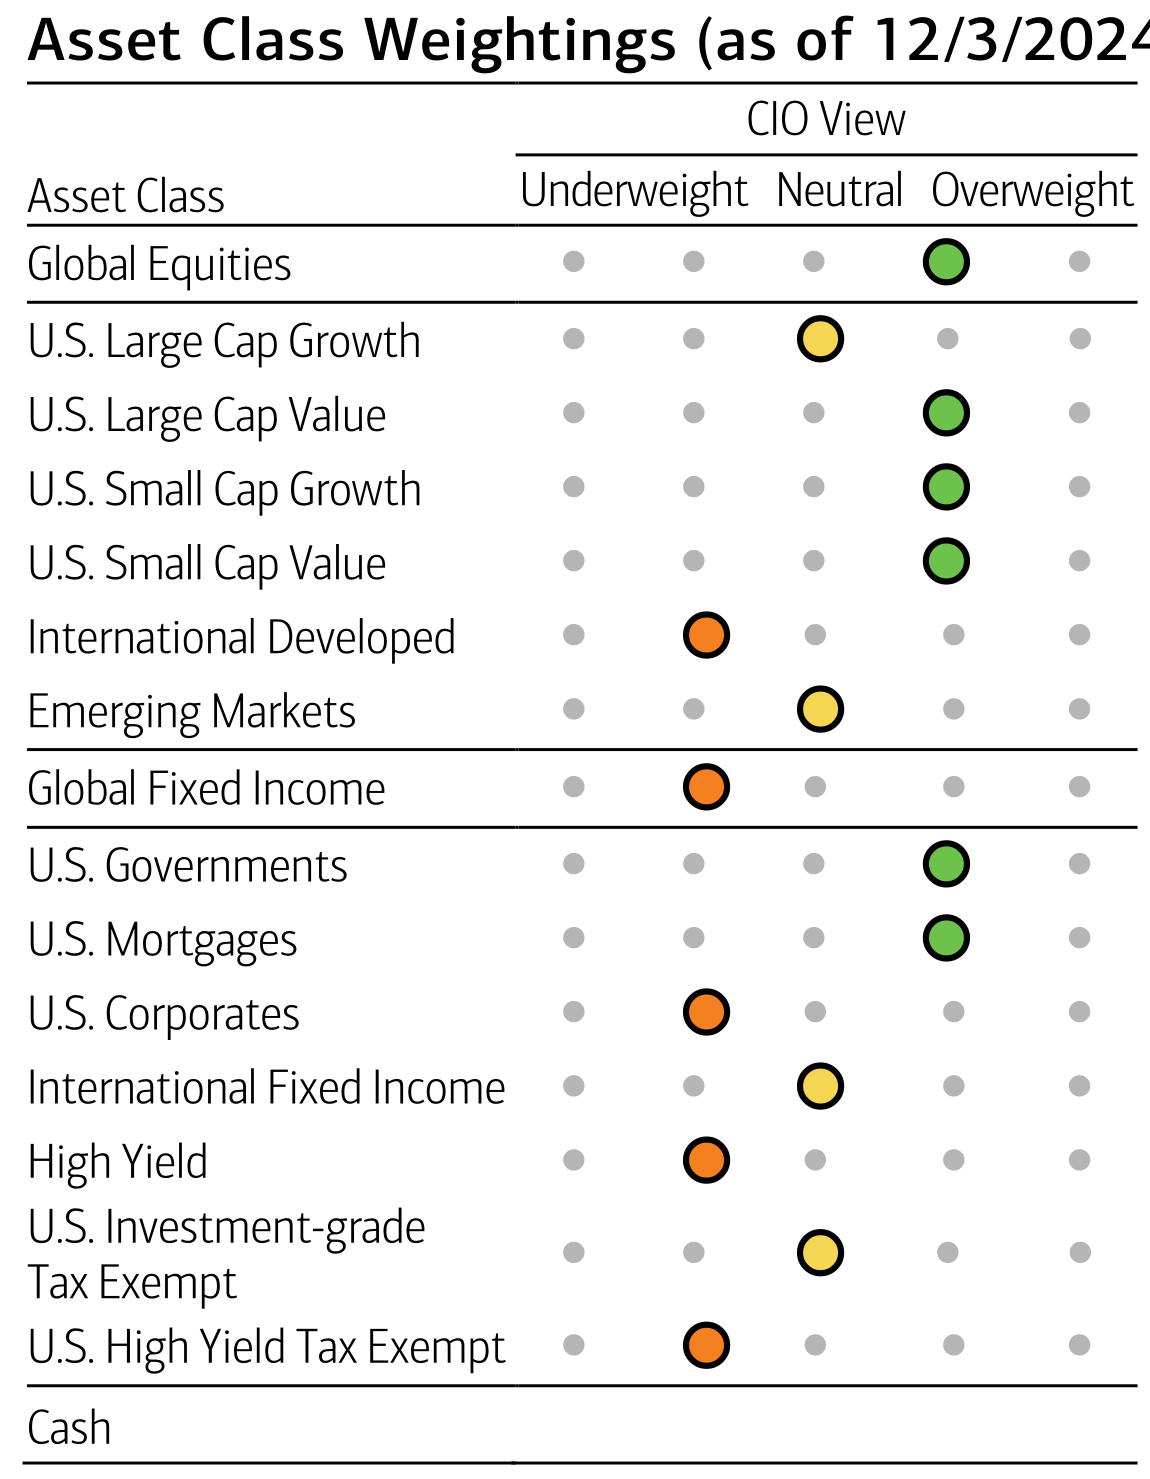
\includegraphics{input/asset_class.png}
\caption{Asset Class Weightings}
\label{fig:asset_class}
\end{figure}

The user will simply define the following data to extract: ``Asset Class Weightings (as of 12/3/2024) in a scale from $-2$ to $2$''. In that way, we expect that ``Underweight'' will be mapped to $-2$, ``Neutral'' to $0$ and ``Overweight'' to $2$ with some values in between.

\begin{minted}{python}
extract_prompt = "Asset Class Weightings (as of 12/3/2024) in a scale from -2 to 2"
asset_class_docling = extract_from_doc(extract_prompt, forecast_result_docling, client)
asset_class_md = extract_from_doc(extract_prompt, forecast_result_md, client)
\end{minted}

\begin{minted}{python}
df_md = pd.DataFrame([(f.financial_variable, f.financial_forecast) for f in asset_class_md.forecasts], 
                 columns=['Variable', 'Forecast'])
df_docling = pd.DataFrame([(f.financial_variable, f.financial_forecast) for f in asset_class_docling.forecasts], 
                 columns=['Variable', 'Forecast'])
\end{minted}

We construct a DataFrame to compare the results from MarkItDown and Docling with an added ``true\_value'' column containing the true values from the document, which we extracted manually from the chart. This enables us to calculate accuracy of the structured data extraction task in case.

\begin{minted}{python}
# Create DataFrame with specified columns
df_comparison = pd.DataFrame({
    'variable': df_docling['Variable'].iloc[:-1],
    'markitdown': df_md['Forecast'],
    'docling': df_docling['Forecast'].iloc[:-1],  # Drop last row
    'true_value': [1.0, 0.0, 1.0, 1.0, 1.0, -1.0, 0.0, -1.0, 1.0, 1.0, -1.0, 0.0, -1.0, 0.0, -1.0]
})

display(df_comparison)
\end{minted}

\begin{table*}[h!]
\centering
\begin{tabular}{lrrr}
\toprule
\textbf{Variable} & \textbf{MarkItDown} & \textbf{Docling} & \textbf{True Value} \\
\midrule
Global Equities & 1.0 & 1.0 & 1.0 \\
\rowcolor{lightgreen} U.S. Large Cap Growth & 1.0 & 1.0 & 0.0 \\ % Mismatch
U.S. Large Cap Value & 1.0 & 1.0 & 1.0 \\
U.S. Small Cap Growth & 1.0 & 1.0 & 1.0 \\
U.S. Small Cap Value & 1.0 & 1.0 & 1.0 \\
\rowcolor{lightyellow} International Developed & 1.0 & -1.0 & -1.0 \\
\rowcolor{lightyellow} Emerging Markets & 1.0 & 0.0 & 0.0 \\
Global Fixed Income & -1.0 & -1.0 & -1.0 \\
\rowcolor{lightyellow} U.S. Governments & -1.0 & 1.0 & 1.0 \\ % Mismatch
\rowcolor{lightyellow} U.S. Mortgages & -1.0 & 1.0 & 1.0 \\ % Mismatch
U.S. Corporates & -1.0 & -1.0 & -1.0 \\
\rowcolor{lightyellow} International Fixed Income & -1.0 & 0.0 & 0.0 \\
High Yield & -1.0 & -1.0 & -1.0 \\
\rowcolor{lightyellow} U.S. Investment-grade & -1.0 & 0.0 & 0.0 \\
Tax Exempt U.S. High Yield Tax Exempt & -1.0 & -1.0 & -1.0 \\
\bottomrule
\end{tabular}
\caption{Comparison of Asset Class Weightings Extraction Results. Highlighted rows indicate cases where there is parsed values did not match with true values: Green for Docling, Yellow for MarkItDown.}
\label{tab:asset-class-comparison}
\end{table*}


\begin{minted}{python}
# Calculate accuracy for markitdown and docling
markitdown_accuracy = (df_comparison['markitdown'] == df_comparison['true_value']).mean()
docling_accuracy = (df_comparison['docling'] == df_comparison['true_value']).mean()

print(f"Markitdown accuracy: {markitdown_accuracy:.2%}")
print(f"Docling accuracy: {docling_accuracy:.2%}") 
\end{minted}


\begin{verbatim}
Markitdown accuracy: 53.33%
Docling accuracy: 93.33%
\end{verbatim}


Docling performs significantly better at 93.33\% accuracy missing only one value. MarkItDown achieves 53.33\% accuracy struggling with nuanced asset class weightings. In this case, Docling's structured parsed output did help the LLM to extract the information more accurately compared to MarkItDown's unstructured output. Hence, in this case, the strategy used to parse the data did impact the LLM's ability to extract structured information. Having said that, it is important to mention that a more robust analysis would run data extraction on a larger sample data a number of times across repeated runs to estimate confidence intervals since results are non-deterministic.

What if we wanted to systematically extract all tables from the document? We can use Docling to do that by simply accessing the \texttt{tables} attribute of the \texttt{DocumentConverter} object.

By doing that, we observe that Docling successfully extracted the seven tables from the document exporting tables from top down and left to right in order of appearance in the document.
Below, we display the first and the last tables. We can see the first table successfully extracted for Equities forecasts, as the last table, which contains CIO Equity Sector Views.
\begin{minted}[highlightlines={20, 21, 22}]{python}
from pathlib import Path
import pandas as pd
from docling.document_converter import DocumentConverter

def convert_and_export_tables(file_path: Path) -> list[pd.DataFrame]:
    """
    Convert document and export tables to DataFrames.
    
    Args:
        file_path: Path to input document
        
    Returns:
        List of pandas DataFrames containing the tables
    """
    doc_converter = DocumentConverter()    
    conv_res = doc_converter.convert(file_path)
    
    tables = []
    # Export tables
    for table in conv_res.document.tables:
        table_df: pd.DataFrame = table.export_to_dataframe()
        tables.append(table_df)
    
    return tables
\end{minted}

\begin{minted}{python}
# Convert and export tables
tables = convert_and_export_tables(Path(FORECAST_FILE_PATH))

print(f"Number of tables extracted: {len(tables)}")
\end{minted}

\begin{verbatim}
Number of tables extracted: 7
\end{verbatim}

\begin{minted}{python}
display(tables[0])
\end{minted}

\begin{table}[H]
\centering
\begin{tabular}{lrrrr}
\hline
 & Current & WTD & MTD & YTD \\
\hline
DJIA & 43,828.06 & -1.8 & -2.3 & 18.4 \\
NASDAQ & 19,926.72 & 0.4 & 3.7 & 33.7 \\
S\&P 500 & 6,051.09 & -0.6 & 0.4 & 28.6 \\
S\&P 400 Mid Cap & 3,277.20 & -1.6 & -2.6 & 19.5 \\
Russell 2000 & 2,346.90 & -2.5 & -3.5 & 17.3 \\
MSCI World & 3,817.24 & -1.0 & 0.2 & 22.1 \\
MSCI EAFE & 2,319.05 & -1.5 & 0.2 & 6.4 \\
MSCI Emerging Markets & 1,107.01 & 0.3 & 2.7 & 10.6 \\
\hline
\end{tabular}
\caption{Market Performance Summary (Total Return in USD \%)}
\label{tab:market-performance}
\end{table}

\begin{minted}{python}
display(tables[6])
\end{minted}

\begin{table}[H]
\centering
\begin{tabular}{lll}
\hline
Sector & CIO View \\
\hline
Utilities & Slight overweight \\
Financials & Slight overweight \\
Healthcare & Slight overweight \\
Consumer Discretionary & Slight overweight \\
Information Technology & Neutral \\
Communication Services & Neutral \\
Industrials & Neutral \\
Real Estate & Neutral \\
Energy & Slight underweight \\
Materials & Slight underweight \\
Consumer Staples & Underweight \\
\hline
\end{tabular}
\caption{Sector Views and Recommendations}
\label{tab:sector-views}
\end{table}

Coming back to MarkItDown, one interesting feature to explore is the ability to extract information from images by passing an image capable LLM model to its constructor.

\begin{minted}{python}
md_llm = MarkItDown(llm_client=client, llm_model="gpt-4o-mini")
\end{minted}

\begin{minted}{python}
result = md_llm.convert("../data/input/forecast.png")
\end{minted}

\begin{minted}{python}
display(Markdown(result.text_content))
\end{minted}
%OK

Here's the description we obtain from the image of our input document~\sidenote{Behind the scenes, MarkitDown is simply passing the following prompt to the LLM: "Write a detailed caption for this image."}.

\begin{verbatim}
Markets in Review: Economic Forecasts and Asset Class Weightings (as of 12/13/2024)

This detailed market overview presents key performance metrics and economic forecasts as of December 13, 2024.

Equities Overview:
- Total Returns: Highlights returns for major indices such as the DJIA (18.4% YTD), NASDAQ (33.7% YTD), and S&P 500 (28.6% YTD), showcasing strong performance across the board.
- Forecasts: Economic indicators reveal a projected real global GDP growth of 3.1%, with inflation rates expected to stabilize around 2.2% in 2025. Unemployment rates are anticipated to remain low at 4.4%.

Fixed Income:
- Focuses on various segments, including Corporate & Government bonds, which offer an annualized return of 4.66% and indicate shifting trends in interest rates over 2-Year (4.25%) and 10-Year (4.03%) bonds.

Commodities & Currencies:
- Commodities such as crude oil and gold show varied performance, with oil increasing by 4.8% and gold prices sitting at $2,648.23 per ounce.
- Currency metrics highlight the Euro and USD trends over the past year.

S&P Sector Returns:
- A quick reference for sector performance indicates a significant 2.5% return in Communication Services, while other sectors like Consumer Staples and Materials display minor fluctuations.

CIO Asset Class Weightings:
- Emphasizes strategic asset allocation recommendations which are crucial for an investor's portfolio. Underweight positions in U.S. Small Cap Growth and International Developed contrast with overweight positions in certain sectors such as Utilities and Financials, signaling tactical shifts based on ongoing economic assessments.

Note: This summary is sourced from BofA Global Research and aims to provide a comprehensive view of current market conditions and forecasts to assist investors in making informed decisions.
\end{verbatim}

Overall, the description is somewhat accurate but it contains a few inaccuracies including~\sidenote{Arguably, the description's inaccuracies is a direct a consequence of the underlying LLM model's inability to process the image.}:

\begin{itemize}
    \item For the sector weightings, the description states there are ``underweight positions in U.S. Small Cap Growth'' but looking at the Asset Class Weightings chart, U.S. Small Cap Growth actually shows an overweight position (green circle).
    \item The description mentions ``overweight positions in certain sectors such as Utilities and Financials'' but looking at the CIO Equity Sector Views, both these sectors show neutral positions, not overweight positions.
    \item For fixed income, the description cites a ``10-Year (4.03\%)'' yield, but the image shows the 30-Year Yield at 4.03\%, while the 10-Year Yield is actually 4.40\%.
\end{itemize}

We have covered MarkitDown and Docling as examples of open source tools that can help developers parse input data into a suitable format to LLMs. Other relevant open source tools worth mentioning include:
\begin{itemize}
    \item Unstructured \sidecite{unstructured2024github}: A Python library for unstructured data extraction.
    \item FireCrawl \sidecite{mendable2024firecrawl}: A Fast and Efficient Web Crawler for LLM Training Data.
    \item LlamaParse \sidecite{llamaparse2024github}: Llamaindex's data parsing solution.
\end{itemize}

The choice of tool depends on the specific requirements of the application and the nature of the input data. This choice should be taken as a critical decision of any data intensive LLM-based application and deserves dedicated research and evidence-based experimentation early-on in the development cycle.

Now how do we add parsed data to an LLM so it can provide contextually relevant up-to-date answer? One answer is via RAGs, the topic of our next section.
%OK

\section{Retrieval-Augmented Generation\index{Retrieval-Augmented Generation (RAG)}}

What happens if we asked ChatGPT\index{ChatGPT} who's the author of the book ``Taming LLMs''?

\begin{minted}{python}
from dotenv import load_dotenv
import os

# Load environment variables from .env file
load_dotenv()

from openai import OpenAI
client = OpenAI()
model = "gpt-4o-mini"
\end{minted}

\begin{minted}{python}
question = "Who's the Author of the Book Taming LLMs?"
\end{minted}

\begin{minted}{python}
response = client.chat.completions.parse(
    model="gpt-4o-mini",
    messages=[
        {"role": "user", "content": question}
    ]
)
response.choices[0].message.content
\end{minted}
\begin{verbatim}
The book "Taming LLMs" is authored by G. Arulkumaran, H. M. B. P. D. Karthikeyan, and I. A. M. Almasri. If you need more information about the book or its contents, feel free to ask!
\end{verbatim}
%OK


Turns out ChatGPT hallucinates. A quick web search on the before mentioned authors yields no results. In fact, those authors names are made up~\sidenote{Of course the correct answer is yours truly, ``Tharsis Souza''.}. 

LLMs only have access to the information they have been trained on, which of course have been fixed at a point in time. Hence, LLMs operate with stale data~\sidenote{There is evidence that LLM's providers' reported date cutoffs differ from effective, observed date cutoffs revealing that not only LLMs inherently work with stale data but that knowledge cutoff itself is not simple to define as one would expect~\cite{cheng2024dateddatatracingknowledge}.}. The problem gets exacerbated by the fact that LLMs are trained to provide an answer even if the answer is unknown by them, hence leading to hallucinations. 

One solution to this problem is to use a retrieval system to fetch information from a knowledge base to provide recent and relevant context to user queries using so-called Retrieval Augmented Generation (RAG) system.

RAG utilizes a retrieval system to fetch external knowledge and augment LLM's context. It is a useful technique for building LLM applications that require domain-specific information or knowledge-intensive tasks \sidecite{lewis2021retrievalaugmentedgenerationknowledgeintensivenlp}. It has also proved effective in mitigating LLMs hallucinations \sidecite{10.1145/3589334.3645481, ni-etal-2024-llms}.

In the above example, a RAG would help with hallucinations by grounding the LLM's response to information provided in the knowledge base. Additional common use cases of RAG systems include:

\begin{enumerate}
    \item \textbf{Enterprise Knowledge Management}~\sidenote{This short paper \cite{bruckhaus2024ragdoesworkenterprises} covers challenges in deploying RAGs in enterprises including data security, scalability and integration issues.}: RAG enables organizations to synthesize answers from diverse internal data sources like documents, databases, and communication channels. This creates a unified knowledge interface that can accurately answer questions using the organization's own data.
    \item \textbf{Document Processing and Analysis}: RAG excels at extracting and analyzing information from complex documents like financial reports, presentations, and spreadsheets. The system can enable LLMs to understand context and relationships across different document types and formats.
    \item \textbf{Intelligent Customer Support}: By combining knowledge bases with conversational abilities, RAG powers chatbots and support systems that can maintain context across chat history, provide accurate responses, and handle complex customer queries while reducing hallucinations.
    \item \textbf{Domain-Specific Applications}: RAG allows LLMs to be equipped with specialized knowledge in fields like medicine, law, or engineering by retrieving information from domain-specific literature, regulations, and technical documentation. This enables accurate responses aligned with professional standards and current best practices.
    \item \textbf{Code Documentation and Technical Support}~\sidenote[][*-1]{An interesting open source parser that enables this use case is \texttt{Repomix}, a tool that can convert an entire codebase into LLM digestable format: \url{https://github.com/yamadashy/repomix}}: RAG can help developers by retrieving relevant code examples, API documentation, and best practices from repositories and documentation, which often suffer updates frequently, enabling more accurate and contextual coding assistance.
\end{enumerate}
%OK


If LLMs alone work on stale, general-purpose data with the added challenge of being prone to hallucinations, RAG systems serve as an added capability enabling LLMs to work on recent, domain-specific knowledge increasing the likelihood of LLMs to provide responses that are factual and relevant to user's queries.
\subsection{RAG Pipeline}

RAG architectures vary but they all share the same goal: To retrieve relevant information from a knowledge base to maximize the LLM's ability to effectively and accurately respond to prompts, particularly when the answer requires out-of-training data.

We will introduce key components of a RAG system one by one leading to a full canonical RAG pipeline at the end that ultimately will be used to answer our original question ``Who's the author of the book Taming LLMs?'', accurately.

The following basic components will be introduced (see Figure \ref{fig:rag_pipeline} for a visual representation):
\begin{itemize}
    \item Vector Database
    \begin{itemize}
        \item Embeddings
        \item Indexing
    \end{itemize}
    \item Retrieval System including re-ranking
    \item LLM Augmented Generation via in-context learning
\end{itemize}

Data extraction, parsing and chunking are also part of a canonical pipeline as we prepare the knowledge base. Those are concepts we explored in detail in Sections \ref{parsing} and \ref{chunking}, hence we will be succinct here. We will start by preparing the knowledge base.

\begin{figure}[H]
\centering
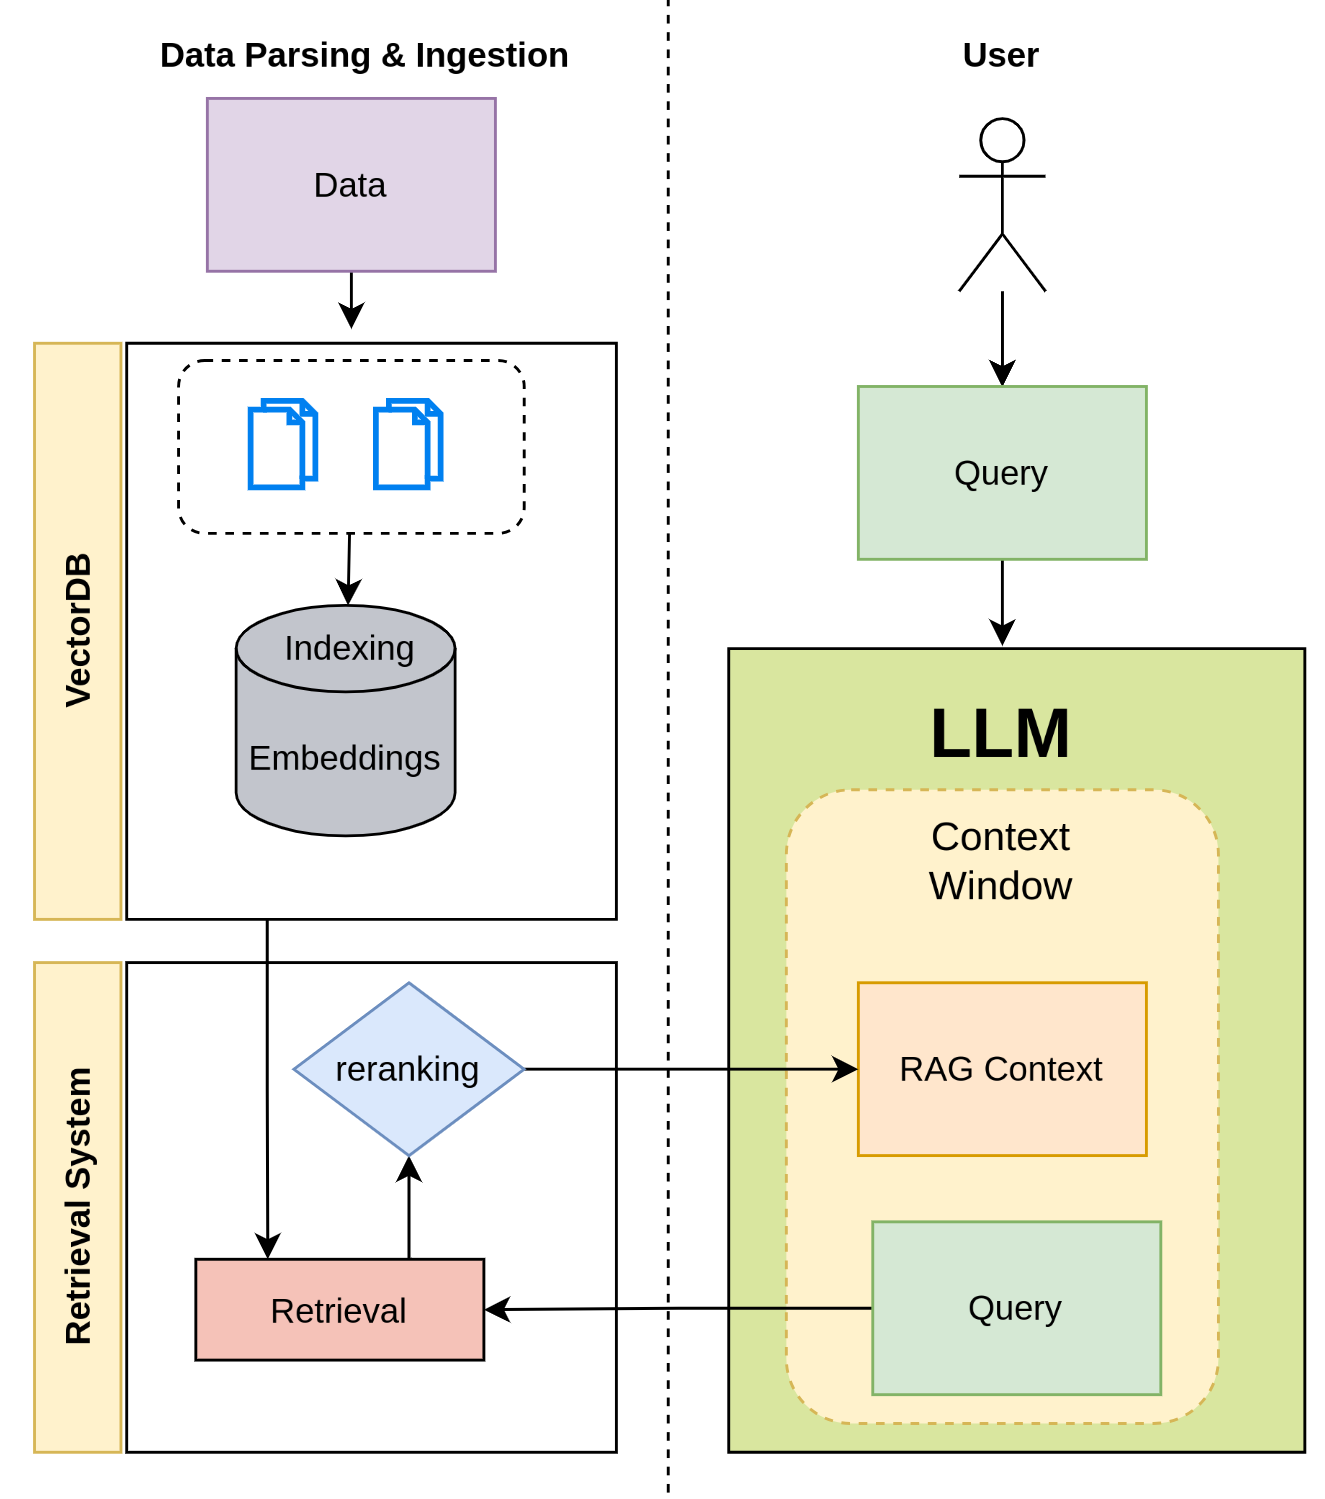
\includegraphics[scale=0.99]{input/rag.png}
\caption{Simplified RAG Pipeline including a Vector Database with Embeddings and Indexing, a Retrieval System including re-ranking with LLM Augmented Generation via In-Context Learning.}
\label{fig:rag_pipeline}
\end{figure}

\subsubsection{Preparing the Knowledge Base}

Every RAG system requires a knowledge base. In our case, the knowledge base is a set of documents that we equip the LLM with to answer our authorship question.

Hence, we will compose our knowledge base by adding the web version of (some of the chapters of) the book ``Taming LLMs'', namely:
\begin{itemize}
    \item Introduction
    \item Structured Output
    \item Input (this very chapter)
\end{itemize}

\begin{minted}{python}
book_url = "https://www.tamingllms.com/"
chapters = ["markdown/intro.html",
            "notebooks/structured_output.html",
            "notebooks/input.html"]

chapter_urls = [f"{book_url}/{chapter}" for chapter in chapters]
chapter_ids = [chapter.split("/")[-1].replace(".html", "") for chapter in chapters]
\end{minted}

We use \texttt{Docling} to download the chapters from the web and parse them as markdown files.

\begin{minted}{python}
chapters = [converter.convert(chapter_url).document.export_to_markdown() for chapter_url in chapter_urls]
\end{minted}
Now we are ready to store the chapters in a vector database to enable the construction of a retrieval system.

\subsubsection{Vector Database\index{VectorDB}}

Vector databases are specialized databases designed to store and retrieve high-dimensional vectors, which are mathematical representations of data like text, images, or audio. These databases are optimized for similarity search operations, making them ideal for embeddings-based retrieval systems.

A typical pipeline involving a vector database includes the following:

\begin{enumerate}
    \item Input data is converted into ``documents'' forming a collection representing our knowledge base
    \item Each document is converted into an embedding which are stored in the vector database
    \item Embeddings are indexed in the vector database for efficient similarity search
    \item The vector database is queried to retrieve the most relevant documents
    \item The retrieved documents are used to answer questions
\end{enumerate}

Vector databases are not a mandatory component of RAG systems. In fact, we can use a simple list of strings to store the chapters (or their chunks) and then use the LLM to answer questions about the document. However, vector databases are useful for RAG applications as they enable:
\begin{itemize}
    \item Fast similarity search for finding relevant context
    \item Efficient storage of document embeddings
    \item Scalable retrieval for large document collections
    \item Flexible querying with metadata filters
\end{itemize}

In that way, RAG applications can be seen as a retrieval system that uses a vector database to store and retrieve embeddings of documents, which in turn are used to augment LLMs with contextually relevant information as we will see in the next sections.

Here, we will use ChromaDB \sidecite{chromadb2024docs} as an example~\sidenote{Other notable vector databases include Weaviate, FAISS, and Milvus.} of an open source vector database but key features and concepts we cover are applicable to other vector databases, in general.

ChromaDB\index{ChromaDB} is a popular open-source vector database that offers:
\begin{itemize}
    \item Efficient storage and retrieval of embeddings
    \item Support for metadata and filtering
    \item Easy integration with Python applications
    \item In-memory and persistent storage options
    \item Support for multiple distance metrics
\end{itemize}

In ChromaDB, we can create a vector database client as follows.

\begin{minted}{python}
import chromadb
chroma_client = chromadb.Client()
\end{minted}

This will create a vector database in memory~\sidenote{We can also create a persistent vector database by specifying a path to a directory or alternatively by using a cloud-based vector database service like AWS, Azure or GCP. We will use a vector database in memory for this example.}.

Next, we create a collection to store the embeddings of the chapters. And add our chapters as documents to the collection as follows.

\begin{minted}{python}
collection = chroma_client.create_collection(name="taming_llms")

collection.add(
    documents=chapters,
    ids=chapter_ids
)
\end{minted}

We are ready to query the collection. We write a simple function that takes the collection, input query and number of retrieved results as argument and returns the retrieved documents.

\begin{minted}{python}
def query_collection(collection, query_text, n_results=3):
    results = collection.query(
        query_texts=[query_text],
        n_results=n_results
    )
    return results
\end{minted}
We write a simple query, enquiring the purpose of the book.

\begin{minted}{python}
q = "What is the purpose of this book?"
res = query_collection(collection, q)
res.get("ids")
\end{minted}

\begin{verbatim}
[['intro', 'input', 'structured_output']]
\end{verbatim}

We obtain an object that contains several attributes including:
\begin{itemize}
    \item \texttt{documents}: The actual documents retrieved from the collection, i.e. the chapters 
    \item \texttt{ids}: The ids of the documents retrieved from the collection
    \item \texttt{distances}: The distances of the documents to the query vector
\end{itemize}

We can see that the chapters ``Introduction'', ``Input'' and ``Structured Output'' are retrieved from the collection ordered by their distance to the query vector, in increasing order.

We observe that the Introduction chapter is the most relevant one as it ranks first, followed by the Input and Structured Output chapters. Indeed, the purpose of the book is included in the Introduction chapter demonstrating the retrieval system successfully retrieved the most relevant document to the input query, in this simple example.

In order to understand how the retrieval system works and how the ``distance to the query vector'' is computed, we need to understand how embeddings are created and how documents are indexed.
%OK


\paragraph{Embeddings\index{Embeddings}} are numerical representations of data (including text, images, audio, etc.) that capture meaning, allowing machines to process data quantitatively. Each embedding can be represented as a vector of floating-point numbers such that embedded data with similar meanings produce similar, i.e. close, vectors \sidenote{Bengio et al. \cite{bengio2014representationlearningreviewnew} provide serves as an excellent reference for representation learning in general including embeddings. OpenAI provides a good intro to Embeddings for developers \cite{openai2024embeddings}}.

For text data, small distances among embeddings suggest high semantic relatedness and large distances suggest low semantic relatedness among the embedded texts. HuggingFace provides a leaderboard of embeddings models \sidecite{huggingface2024mteb}, which are ranked by dimensions such as classification, clustering and reranking performance.

Behind the scenes, ChromaDB is using the model \texttt{all-MiniLM-L6-v2} by default \sidenote{ChromaDB enables custom \href{https://docs.trychroma.com/docs/embeddings/embedding-functions}{embedding functions} and provides a list of wrappers around commonly used embedding models and APIs} to create embeddings for the input documents and the query (see Figure \ref{embedding}). This model is available in \texttt{sentence\_transformers} \sidecite{sentencetransformers2024website}. Let's see how it works.

%OK


\begin{figure}[H]
\centering
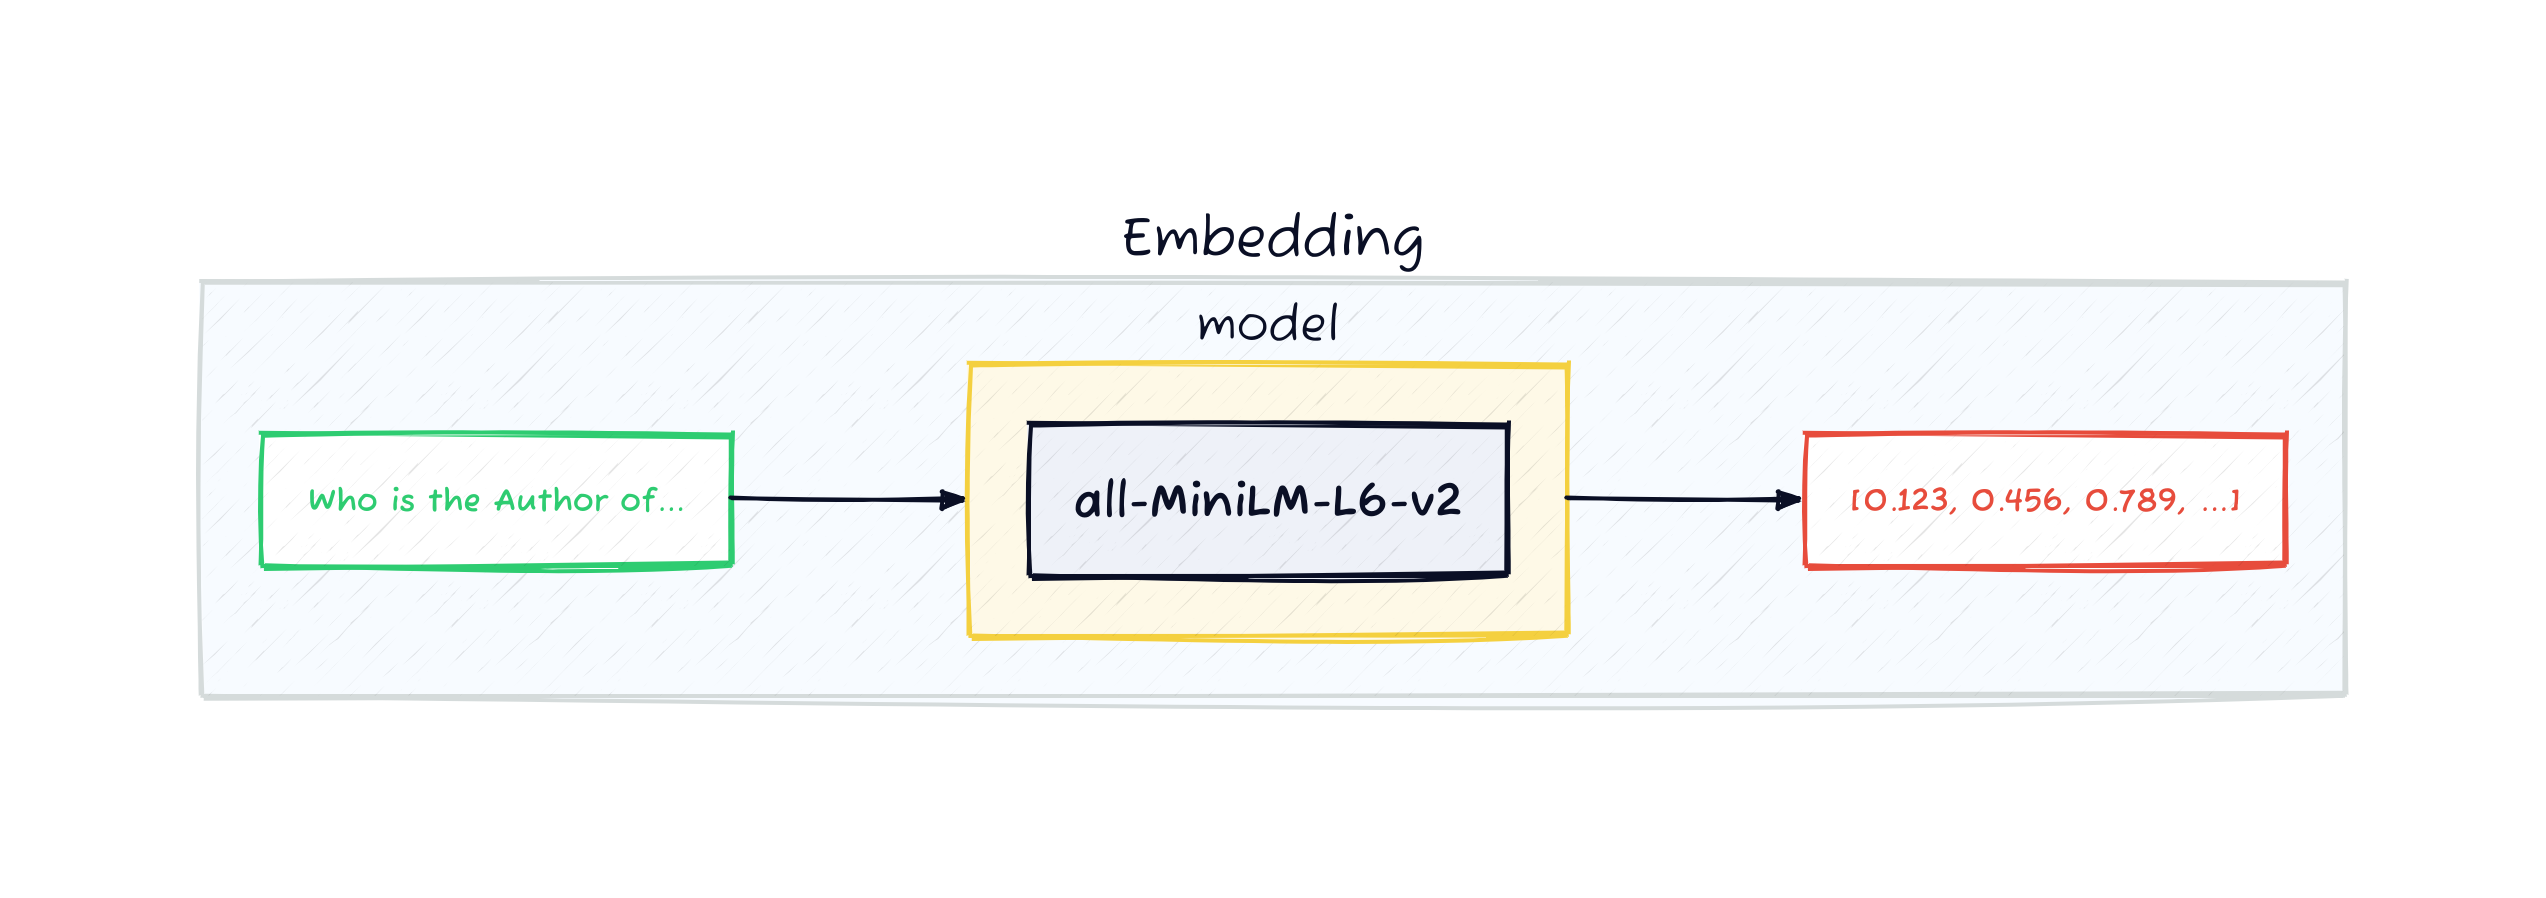
\includegraphics[scale=0.7]{input/embedding.png}
\caption{Embedding: From text to vectors.}
\label{embedding}
\end{figure}

\begin{minted}{python}
from sentence_transformers import SentenceTransformer

embedding_model = SentenceTransformer('all-MiniLM-L6-v2')
\end{minted}

We replicate what ChromaDB did by embedding our chapters as well as input query using sentence transformers.

\begin{minted}{python}
q = "What is the purpose of this book?"
docs_to_embed = [q] + chapters
embeddings = embedding_model.encode(docs_to_embed)
print(embeddings.shape)
\end{minted}

\begin{verbatim}
(4, 384)
\end{verbatim}

As a result, we obtain four 384-dimensional vectors representing our embeddings (one for each of the three chapters and one for the input query).

Now we can calculate similarity among the embeddings. By default, sentence transformers uses cosine similarity as similarity metric.

\begin{minted}{python}
similarities = embedding_model.similarity(embeddings, embeddings)
similarities
\end{minted}

\begin{verbatim}
tensor([[1.0000, 0.4402, 0.3022, 0.4028],
        [0.4402, 1.0000, 0.6606, 0.5807],
        [0.3022, 0.6606, 1.0000, 0.6313],
        [0.4028, 0.5807, 0.6313, 1.0000]])
\end{verbatim}

Let's visualize the similarity matrix to better understand the relationships between our documents in Figure \ref{similarities}. The top row of the matrix represents the similarity of the input query against all chapters. That's exactly what we previously obtained by querying ChromaDB which returned a response with documents ranked by similarity to input query. As expected, the Introduction chapter is the most similar to the input query followed by the Input and Structured Output chapters, as we previously observed with ChromaDB.

\begin{figure}[H]
\centering
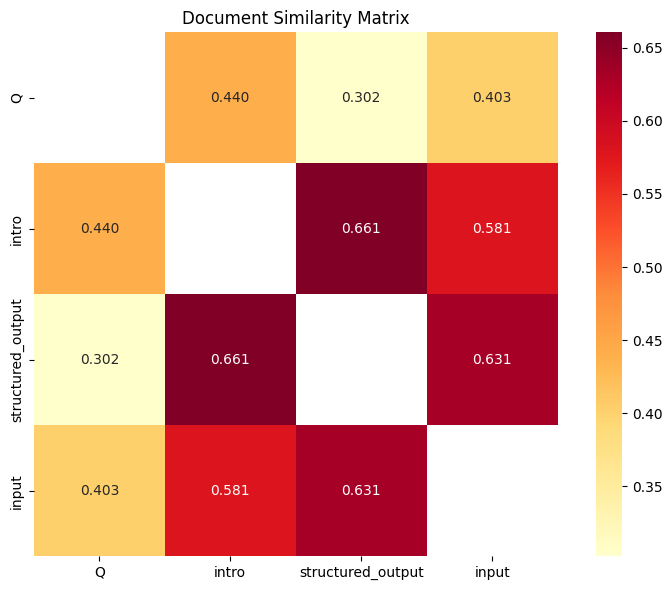
\includegraphics[scale=0.75]{input/similarity.png}
\caption{Similarity matrix heatmap showing relationships among query and chapters.}
\label{similarities}
\end{figure}


Calculating similarity among embeddings can become computationally intensive if brute force is used, i.e. pair-wise computation, as the number of documents grows in the knowledge base. Indexing is a technique to help address this challenge.

\paragraph{Indexing\index{Indexing}} is an optimization technique that makes similarity searches faster and more efficient.

Without indexing, finding similar vectors would require an exhaustive search - comparing a query vector against every single vector in the database. For large datasets, this becomes prohibitively slow.

Common indexing strategies include:

\begin{enumerate}
    \item \textbf{Tree-based Indexes}
    \begin{itemize}
        \item Examples include KD-trees and Ball trees
        \item Work by partitioning the vector space into hierarchical regions  
        \item Effective for low-dimensional data but suffer from the ``curse of dimensionality''
    \end{itemize}

    \item \textbf{Graph-based Indexes}
    \begin{itemize}
        \item HNSW~\sidecite{oracle_hierarchical_indexes} (Hierarchical Navigable Small World) is a prominent example
        \item Creates a multi-layered graph structure for navigation
        \item Offers excellent search speed but requires more memory
    \end{itemize}

    \item \textbf{LSH~\sidecite{jafari2021surveylocalitysensitivehashing} (Locality-Sensitive Hashing)}
    \begin{itemize}
        \item Uses hash functions that map similar vectors to the same buckets
        \item More memory-efficient than graph-based methods
        \item May sacrifice some accuracy for performance
    \end{itemize}

    \item \textbf{Quantization-based Indexes}
    \begin{itemize}
        \item Product Quantization compresses vectors by encoding them into discrete values
        \item Reduces memory footprint significantly
        \item Good balance between accuracy and resource usage
    \end{itemize}
\end{enumerate}
HNSW is the underlying library for ChromaDB vector indexing and search \sidecite{chromadb2024hnsw}. HNSW provides fast searches with high accuracy but uses more memory. LSH and quantization methods offer better memory efficiency but may sacrifice some precision.

But is the combination of indexing and basic embeddings-based similarity sufficient to retrieve relevant documents? Often not, as we will see next, as we cover reranking technique.

\subsection{Reranking\index{Reranking}}

Let's go back to querying our vector database.

First, we write a query about how to get structured output from LLMs. Successfully retrieving the "Structured Output" chapter from the book as top result.

\begin{minted}{python}
q = "How to get structured output from LLMs?"
res = query_collection(collection, q)
res.get("ids")
\end{minted}

\begin{verbatim}
[['structured_output', 'input', 'intro']]
\end{verbatim}

Next, we would like to obtain a tutorial on \texttt{Docling}, a tool we covered in this very chapter. However, we fail to obtain the correct chapter and instead obtain the "Introduction" chapter as a result.

\begin{minted}{python}
q = "Docling tutorial"
res = query_collection(collection, q)
res.get("ids")
\end{minted}

\begin{verbatim}
[['intro', 'input', 'structured_output']]
\end{verbatim}

Retrieval systems solely based on vector similarity search might miss semantic relevance \sidecite{Lin2024, li2021embeddingbasedproductretrievaltaobao}. That brings the need for techniques that can improve accuracy of the retrieval system. One such technique is re-ranking~\sidecite{nvidia2024reranking}.

Re-ranking is a method that can improve accuracy of the retrieval system by re-ranking the retrieved documents based on their relevance to the input query.

In the following, we will use the \texttt{sentence\_transformers} library~\sidecite{sbert2024website} to re-rank the retrieved documents based on their relevance to the input query. We utilize the \texttt{CrossEncoder} model to re-rank the documents~\sidecite{tran2021rerankmatchsemisupervisedlearningsemanticsoriented}. Cross-Encoder models are more accurate at judging relevance at the cost of speed compared to basic vector-based similarity.

We can implement a reranking step in a RAG system using a Cross-Encoder model in the following steps:

1. First, we initialize the Cross-Encoder\index{Cross-Encoder} model:
\begin{minted}{python}
from sentence_transformers import CrossEncoder
model = CrossEncoder('cross-encoder/ms-marco-MiniLM-L-6-v2', max_length=512)
\end{minted}
\begin{itemize}
    \item Uses the \texttt{ms-marco-MiniLM-L-6-v2} model, which is specifically trained for passage reranking
    \item Sets a maximum sequence length of 512 tokens
    \item This model is designed to score the relevance between query-document pairs
\end{itemize}
2. Then we perform the reranking:
\begin{minted}{python}
scores = model.predict([(q, doc) for doc in res["documents"][0]])
\end{minted}
\begin{itemize}
    \item Creates pairs of (query, document) for each retrieved document
    \item The model predicts relevance scores for each pair
    \item Higher scores indicate better semantic match between query and document
\end{itemize}

3. Finally, we select the best match:
\begin{minted}{python}
print(res["documents"][0][np.argmax(scores)])
\end{minted}
\begin{itemize}
    \item \texttt{np.argmax(scores)} finds the index of the highest scoring document
    \item Uses that index to retrieve the most relevant document
\end{itemize}

We obtain the following scores for the retrieved documents ("intro", "input", "structured\_output"), the higher the score, the more relevant the document is in relation to the input query.

\begin{verbatim}
array([-8.52623 , -6.328738, -8.750055], dtype=float32)
\end{verbatim}

As a result, we obtain the index of the highest scoring document, which corresponds to the "input" chapter. Hence, the re-ranking step successfully retrieved the correct chapter.

\begin{minted}{python}
print(f"The most relevant document is: {res['ids'][0][np.argmax(scores)]}")
\end{minted}

\begin{verbatim}
The most relevant document is: input
\end{verbatim}

In RAG systems, the idea is to first run semantic similarity on embeddings, which should be fast but potentially inaccurate, and then run reranking from the top-k results, which should be more accurate but slower. By doing so, we can balance the speed and accuracy of the retrieval system.

Hence, instead of going over all retrieved documents:
\begin{minted}{python}
scores = model.predict([(q, doc) for doc in res["documents"][0]])
\end{minted}
We would run reranking on the TOPK results, where TOPK $\ll$ number of documents:
\begin{minted}{python}
scores = model.predict([(q, doc) for doc in res["documents"][0][:TOPK]])
\end{minted}

\subsection{LLMs with RAG}

We are finally ready to use the retrieval system to help the LLM answer our authorship question. A common way to integrate RAGs with LLMs is via in-context learning. With in-context learning the LLM learns from the retrieved documents by providing them in the context window as represented in Figure \ref{fig:incontext}. This is accomplished via a prompt template structure as follows.

\begin{figure}[H]
\centering
\includesvg[scale=0.99]{input/incontext.svg}
\caption{RAG LLM with In-Context Learning}
\label{fig:incontext}
\end{figure}

\begin{minted}{python}
rag_system_prompt_template = f"""
You are a helpful assistant that answers questions based on the provided CONTEXT.

CONTEXT: {context}
"""

user_prompt_template = f"""
QUESTION: {input}
"""
\end{minted}

This prompt strategy demonstrates a common in-context learning~\sidenote{You might ask: How does the in-context content provided interplay with the pre-trained data? ICLR 2024 paper \cite{park2024iclrincontextlearningrepresentations} provides evidence that if we add in-context exemplars wherein a concept plays a different role than what the pre-training data suggests, models reorganize their representations in accordance with these novel semantics.} pattern where retrieved documents are incorporated into the LLM's context to enhance response accuracy and relevance. The prompt structure typically consists of a system prompt that:

\begin{itemize}
    \item Sets clear boundaries for the LLM to use information from the provided context
    \item Includes the retrieved documents as context
\end{itemize}

This approach:
\begin{itemize}
    \item Reduces hallucination by grounding responses in source documents
    \item Improves answer relevance by providing contextually relevant information to the LLM
\end{itemize}
The context variable is typically populated with the highest-scoring document(s) from the retrieval step, while the input variable contains the user's original query.

\begin{minted}{python}
def RAG_qa(client, model, context, input):
    rag_system_prompt_template =  f"""You are a helpful assistant that answers questions based on the provided CONTEXT.

    CONTEXT: {context}
    """
    
    response = client.chat.completions.create(
    model=model,
        messages=[{"role": "system", "content": rag_system_prompt_template},
                 {"role": "user", "content": f"QUESTION: {input}"}]
    )
    return response.choices[0].message.content
\end{minted}

First, we set the LLM.

\begin{minted}{python}
from dotenv import load_dotenv
import os

# Load environment variables from .env file
load_dotenv()

from openai import OpenAI
client = OpenAI()
model = "gpt-4o-mini"
\end{minted}

Then, we run the retrieval step.

\begin{minted}{python}
res = query_collection(collection, q)
\end{minted}

Next, we run the re-ranking step setting it to consider the \texttt{TOPK} retrieved documents.

\begin{minted}{python}
TOPK = 2
scores = model.predict([(q, doc) for doc in res["documents"][0][:TOPK]])
res_reranked = res["documents"][0][np.argmax(scores)]
\end{minted}

We then pass the top document as context and invoke the LLM with our RAG-based template leading to a successful response.

\begin{minted}{python}
answer = RAG_qa(model, res_reranked[0], question)
answer
\end{minted}

\begin{verbatim}
The author of the book "Taming LLMs" is Tharsis Souza.
\end{verbatim}
In this section, we motivated the use of RAGs as a tool to equip LLMs with relevant context and provided a canonical implementation of its core components. RAGs, however, can be implemented in many shapes and forms and entire books have been written about them. We point the user to additional resources if more specialized techniques and architectures are needed \sidecite{10.1007/s10791-009-9096-x, deeplearningai2024rag, kimothi2024simpleguiderag, athinaai2024ragcookbooks, diamant2024ragtechniques, hands-on-llms-book}.

Next, we discuss RAGs challenges and limitations and conclude our RAGs section envisioning their future challenged by the rise of long-context language models.
%OK


\subsection{Challenges and Limitations}

While RAG systems offer powerful capabilities for enhancing LLM responses with external knowledge, they face several significant challenges and limitations that require careful consideration:
 
\textbf{Data Quality and Accuracy}: The effectiveness of RAG systems fundamentally depends on the quality and reliability of their knowledge sources. When these sources contain inaccurate, outdated, biased, or incomplete information, the system's responses become unreliable. This challenge is particularly acute when dealing with rapidly evolving topics or when sourcing information from unverified channels.
 
\textbf{Computational Cost and Latency}: Implementing RAG systems at scale presents computational and operational challenges~\sidenote{This work \cite{jin2024ragcacheefficientknowledgecaching} pinpoints several optimization opportunities to reduce computational and memory costs in RAGs reducing the time to first token by up to 4x and increasing throughput by up to 2.1x compared to benchmarks.}. The process of embedding documents, maintaining vector databases, and performing similarity searches across large knowledge bases demands computational, and operational resources. In real-time applications, these requirements can introduce noticeable latency, potentially degrading the user experience and limiting practical applications.
 
\textbf{Explainability and Evaluation}: The complexity of RAG systems, arising from the intricate interaction between retrieval mechanisms and generative models, makes it difficult to trace and explain their reasoning processes. Traditional evaluation metrics often fail to capture the nuanced aspects of RAG performance, such as contextual relevance and factual consistency. This limitation hampers both system improvement and stakeholder trust. Readers are encouraged to read Chapter \ref{chapter:evals} for general LLM evaluation issues as well as consider tools such as Ragas \sidecite{ragas2024evaluation} for RAG evaluation.
 
\textbf{Hallucination\index{Hallucination} Management}: Though RAG systems help ground LLM responses in source documents, they do not completely eliminate hallucinations. The generative component may still produce content that extrapolates beyond or misinterprets the retrieved context. This risk becomes particularly concerning when the system confidently presents incorrect information with apparent source attribution.

Moreover, recent research has shed light on critical limitations of key techniques used in RAGs systems. A relevant finding pertains to reranking, which has shown \sidecite{jacob2024drowningdocumentsconsequencesscaling}:

\begin{itemize}
\item \textbf{Diminishing Returns}: Performance degrades as the number of documents ($K$) increases, sometimes performing worse than basic retrievers when dealing with large datasets.
\item \textbf{Poor Document Discrimination}: Rerankers can be misled by irrelevant documents, sometimes assigning high scores to content with minimal relevance to the query.
\item \textbf{Consistency Issues}: Performance and relative rankings between different rerankers can vary significantly depending on the number of documents being processed.
\end{itemize}
\subsection{Will RAGs exist in the future?}

This question is posed as we contrast RAGs with LLMs with long-context windows\index{Long-context language models} (LCs).

Recent research has shed light on this specific point \sidecite{li2024retrievalaugmentedgenerationlongcontext} suggesting a trade-off between cost and performance. On the one hand, RAGs can be seen as a cost-effective alternative to LC models:
\begin{itemize}
\item RAGs offer lower computational cost compared to LCs due to the significantly shorter input length required for processing.
\item This cost-efficiency arises because RAG reduces the number of input tokens to LLMs, which in turn reduces overall usage cost.
\end{itemize}

On the other hand, this RAG benefit is achieved at the cost of performance:
\begin{itemize}
\item Recent advancements in LLMs, in particular with Gemini-1.5\index{Gemini} and GPT-4o models\index{GPT}, demonstrate capabilities in understanding long contexts directly, which enables them to outperform RAG in terms of average performance.
\item LC models can process extremely long contexts, such as Gemini 1.5 which can handle up to 1 million tokens, and these models benefit from large-scale pretraining to develop strong long-context capabilities.
\end{itemize}

This cost-performance trade-off is illustrated in Figure \ref{fig:LC}, where LC models outperform RAGs in terms of average performance while RAGs are more cost-effective.

\begin{figure}[H]
\centering
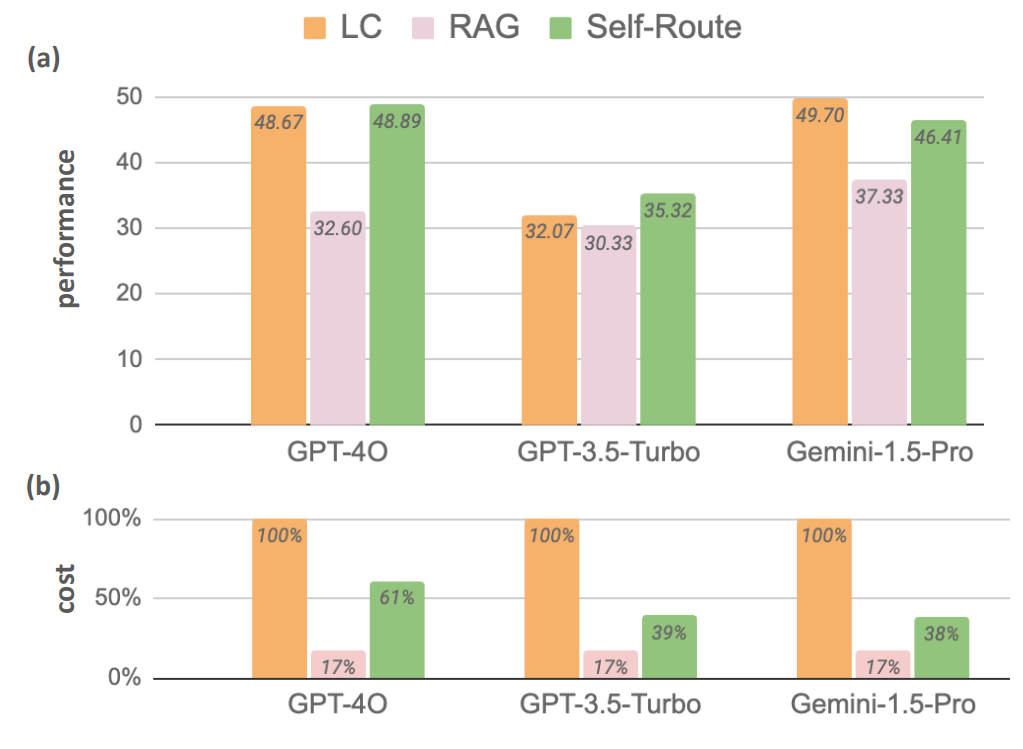
\includegraphics{input/LC.png}
\caption{Long-Context LLMs demonstrate superior performance while RAGs are more cost-effective \cite{li2024retrievalaugmentedgenerationlongcontext}.}
\label{fig:LC}
\end{figure}
Figure \ref{fig:LC} also shows a model called "SELF-ROUTE" which combines RAG and LC by routing queries based on model self-reflection. This is a hybrid approach that reduces computational costs while maintaining performance comparable to LC. The advantage of SELF-ROUTE is most significant for smaller values of $k$, where $k$ is the number of retrieved text chunks, and SELF-ROUTE shows a marked improvement in performance over RAG, while as $k$ increases the performance of RAG and SELF-ROUTE approaches that of LC.

Another example of a hybrid approach that combines the benefits of both LC and RAGs is RetroLLM \sidecite{li2024retrollmempoweringlargelanguage}, which is a unified framework that integrates retrieval and generation into a single process, enabling language models to generate fine-grained evidence directly from a corpus. The key contribution is that this approach delivers those benefits while eliminating the need for a separate retriever, addressing limitations of traditional RAG methods. Experimental results demonstrate RetroLLM's superior performance compared to traditional RAG methods, across both in-domain and out-of-domain tasks. It also achieves a significant reduction in token consumption due to its fine-grained evidence retrieval.

CAG \sidecite{chan2024dontragcacheaugmentedgeneration} is another solution that eliminates the need for RAGs as it proposes cache-augmented generation (CAG). CAG preloads all relevant data into a large language model's extended context window, eliminating the need for real-time retrieval and improving speed and accuracy. This is achieved by precomputing a key-value cache, further optimizing inference time. CAG demonstrates superior performance compared to RAG by achieving higher BERT scores in most evaluated scenarios, indicating better answer quality, and by having significantly reduced generation times. These results suggest that CAG can be both more accurate and more efficient than traditional RAG systems.

An important development in this area is the introduction of LOFT \sidecite{lee2024longcontextlanguagemodelssubsume}, a benchmark to assess this paradigm shift from RAGs to LCs, using real-world tasks requiring context up to millions of tokens. Evidence suggests LCs can deliver performance with simplified pipelines compared to RAGs, particularly for tasking requiring multi-hop reasoning over long contexts when using Chain-of-Thought \sidecite{wei2023chainofthoughtpromptingelicitsreasoning}. However, LCs can still be outperformed by specialized retrievers, in particular Gecko, a specialized model fine-tuned on extensive text retrieval and similarity tasks.

Bottom-line: Do we really need RAGs? The answer is conditional:

\begin{itemize}
\item \textbf{RAG may be relevant when cost-effectiveness is a key requirement} and where the model needs to access vast amounts of external knowledge without incurring high computational expenses. However, as LLMs context window sizes increase and LLMs cost per input token decreases, RAGs may not be as relevant as it was before.
\item \textbf{Long-context LLMs are superior when performance is the primary concern}, and the model needs to handle extensive texts that require deep contextual understanding and reasoning.
\item \textbf{Hybrid approaches are valuable as they combine the strengths of RAG and LC} offering a practical balance between cost and performance, especially for applications where both factors are critical.
\end{itemize}
Ultimately, the choice among RAG, LC, or a hybrid method depends on the specific requirements of the task, available resources, and the acceptable trade-off between cost and performance.

In a later case study, we demonstrate the power of LCs as we construct a Quiz generator with citations over a large knowledge base without the use of chunking nor RAGs.

\section{A Note on Frameworks}

We have covered a few open source tools for parsing data and provided a canonical RAG pipeline directly using an open source VectorDB together with an LLM. There is a growing number of frameworks that offer similar functionality around similar core concepts at a higher level of abstraction. The two most popular ones are \texttt{LangChain}\index{LangChain}~\sidenote{\texttt{LangChain} provides a helpful RAG tutorial by means of an agent-based implementation: \url{https://python.langchain.com/docs/tutorials/rag/}.} and \texttt{LlamaIndex}\index{LlamaIndex}. 

For instance, the code below shows how to use \texttt{LlamaIndex}'s \texttt{LlamaParse} for parsing input documents, which offers support for a wide range of file formats (e.g. .pdf, .pptx, .docx, .xlsx, .html). We observe that the code is very similar to the one we used for \texttt{MarkitDown} and \texttt{Docling}.

\begin{minted}{python}
from llama_parse import LlamaParse

# Initialize the parser
parser = LlamaParse(
    api_key="llx-your-api-key-here",
    result_type="markdown",  # Can be "markdown" or "text"
    verbose=True
)

documents = parser.load_data(["./doc1.pdf", "./doc2.pdf"])
\end{minted}
As another example, the code below replicates our ChromaDB-based retrieval system using \texttt{LlamaIndex} \sidecite{llamaindex2024storing}.

As we can see, similar concepts~\sidenote[][*1]{\texttt{LlamaIndex} demonstrates an alternative to the "in-context learning" approach we have covered by equipping an LLMs with a RAG as a tool via function calling in \url{https://docs.llamaindex.ai/en/stable/understanding/agent/rag_agent/}} are used:
\begin{itemize}
\item Documents to represent elements of the knowledge base
\item Collections to store the documents
\item Indexing of embeddings in the VectorDB and finally
\item Querying the VectorDB to retrieve the documents
\end{itemize}

\begin{minted}{python}
import chromadb
from llama_index.core import VectorStoreIndex, SimpleDirectoryReader
from llama_index.vector_stores.chroma import ChromaVectorStore
from llama_index.core import StorageContext

# load some documents
documents = SimpleDirectoryReader("./data").load_data()

# initialize client, setting path to save data
db = chromadb.PersistentClient(path="./chroma_db")

# create collection
chroma_collection = db.get_or_create_collection("tamingllms")

# assign chroma as the vector_store to the context
vector_store = ChromaVectorStore(chroma_collection=chroma_collection)
storage_context = StorageContext.from_defaults(vector_store=vector_store)

# create your index
index = VectorStoreIndex.from_documents(
    documents, storage_context=storage_context
)

# create a query engine and query
query_engine = index.as_query_engine()
response = query_engine.query("Who is the author of Taming LLMs?")
print(response)
\end{minted}
Frameworks are useful for quickly prototyping RAG systems and for building applications on top of them as they provide a higher level of abstraction and integration with third-party libraries. Further, some frameworks such as LlamaIndex and LangChain also are scoped to provide a production path, offering products that deliver on LLM observability and cloud support, for instance. 

However, more often than not, problems arise when developers either do not understand the underlying concepts or fail to understand the details of the implement behind the abstractions provided by used framework. Therefore, it is recommended to try and start your implementation using lower level tools as much as possible and only when (i) the underlying problem and (ii) the desired solution are well understood, then consider moving to higher level frameworks if really needed.
%OK


\section{Case Studies}

This section presents two case studies to complement topics we have covered in this chapter in the context of managing input data for LLMs.

First, we cover content chunking, in particular Content Chunking\index{Chunking} with Contextual Linking which showcases how intelligent chunking strategies can overcome both context window and output token limitations. This case study illustrates techniques for breaking down and reassembling content while maintaining coherence, enabling the generation of high-quality long-form outputs despite model constraints.

Second, we build a Quiz generator with citations using long context window. Not all knowledge intense applications require RAGs. In this case study, we show how to use long context window as well as some additional input management techniques such as prompt caching for efficiency and reference management to enhance response accuracy and verifiability. These approaches show how to maximize the benefits of larger context models while maintaining response quality.

\subsection{Case Study I: Content Chunking with Contextual Linking}
\label{chunking}
Content chunking is commonly used to breakdown long-form content into smaller, manageable chunks. In the context of RAGs, this can be helpful not only to enable the retrieval system find more contextually relevant documents but also lead to a more cost efficient LLM solution since fewer tokens are processed in the context window. Furthermore, semantic chunking can increase accuracy of RAG systems \sidecite{zenml2024rag}.

Content chunking with contextual linking is a chunking technique that seeks to split input content while keeping chunk-specific context, hence allowing the LLM to maintain coherence and context when generating responses per chunks. In that way, this technique tackles two key problems:
\begin{enumerate}
\item The LLM's inability to process long inputs to do context-size limits
\item The LLM's inability to maintain coherence and context when generating responses per chunks
\end{enumerate}

As a consequence, a third problem is also tackled: LLM's inability to generate long-form content due to the \texttt{max\_output\_tokens} limitation. Since we generate responses per chunk, as we will see later, we end up with a solution that is capable of generating long-form content while maintaining coherence.

We exemplify this technique by following these steps:
\begin{enumerate}
\item \textbf{Chunking the Content}: The input content is split into smaller chunks. This allows the LLM to process each chunk individually, focusing on generating a complete and detailed response for that specific section of the input.

\item \textbf{Maintaining Context}: Each chunk is linked with contextual information from the previous chunks. This helps in maintaining the flow and coherence of the content across multiple chunks.

\item \textbf{Generating Linked Prompts}: For each chunk, a prompt is generated that includes the chunk's content and its context. This prompt is then used to generate the output for that chunk.

\item \textbf{Combining the Outputs}: The outputs of all chunks are combined to form the final long-form content.
\end{enumerate}

Let's examine an example implementation of this technique in the following use case:
\begin{itemize}
\item Goal: Generate a long-form report analyzing a company's financial statement.
\item Input: A company's 10K SEC filing.
\end{itemize}

\begin{figure}[H]
\centering
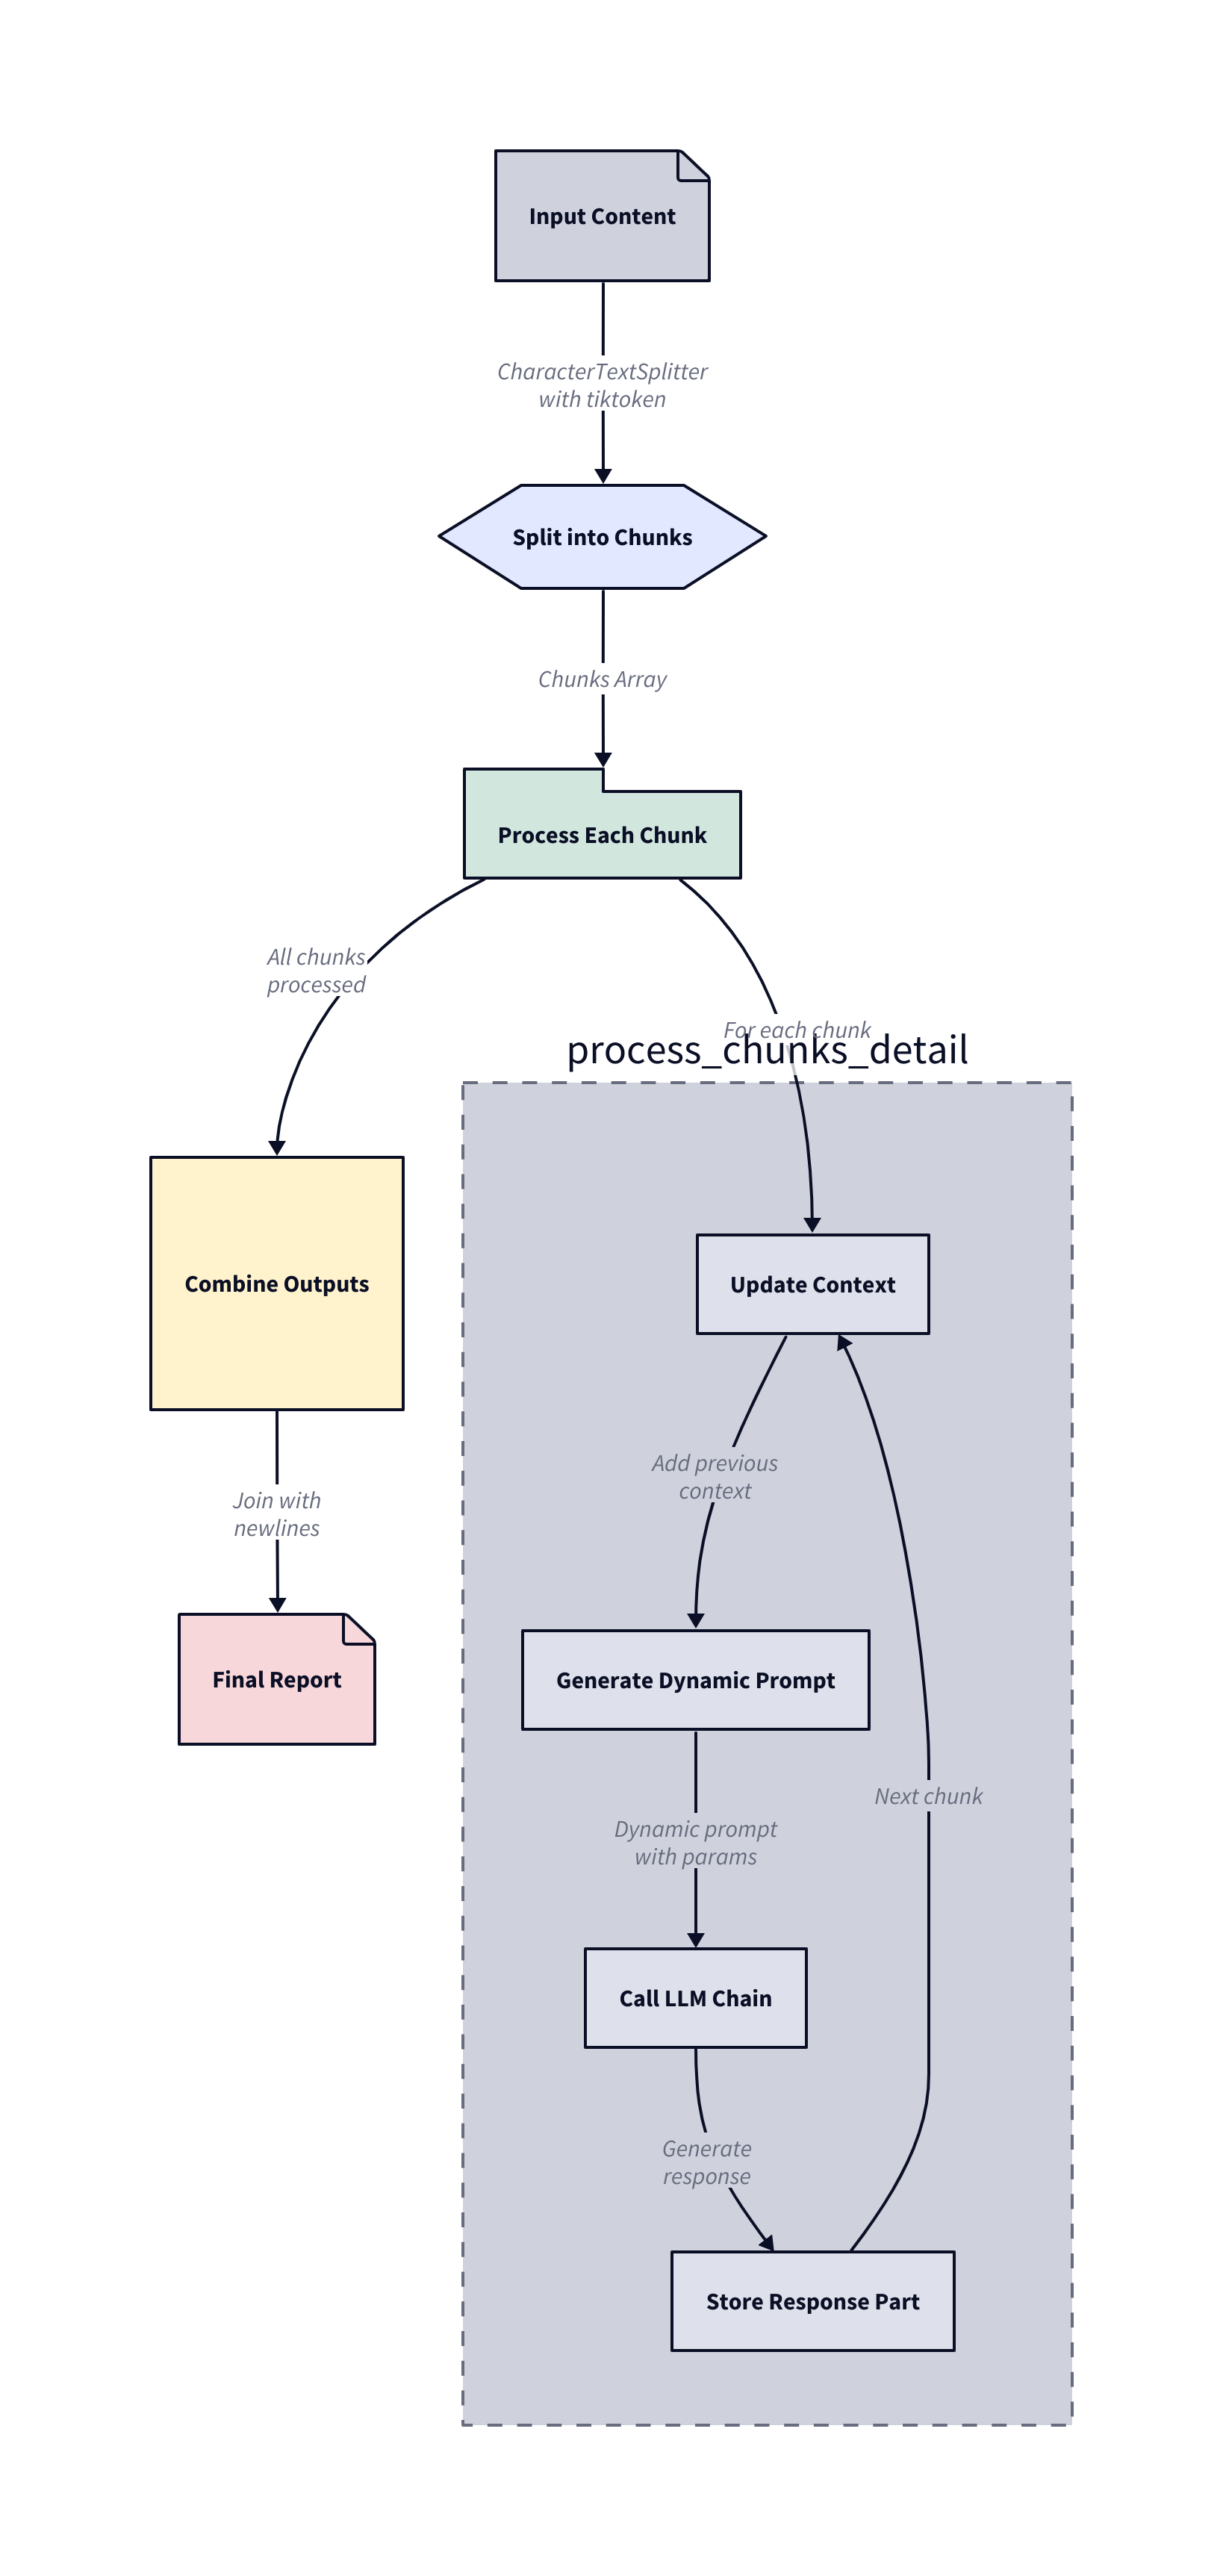
\includegraphics[scale=0.55]{structured_output/diagram1.png}
\caption{Content Chunking with Contextual Linking Schematic Representation.}
\label{content-chunking-with-contextual-linking}
\end{figure}

The diagram in Figure~\ref{content-chunking-with-contextual-linking} illustrates the process we will follow for handling long-form content generation with Large Language Models through ``Content Chunking with Contextual Linking.'' It shows how input content is first split into manageable chunks using a chunking function (e.g. \texttt{CharacterTextSplitter}~\sidenote{A list of text splitters available in \texttt{LangChain} is available at \url{https://python.langchain.com/docs/concepts/text_splitters/}} with \texttt{tiktoken} tokenizer), then each chunk is processed sequentially while maintaining context from previous chunks. For each chunk, the system updates the context, generates a dynamic prompt with specific parameters, makes a call to the LLM chain, and stores the response. After all chunks are processed, the individual responses are combined with newlines to create the final report, effectively working around the token limit constraints of LLMs while maintaining coherence across the generated content.
\paragraph{Step 1: Chunking the Content}

There are different methods for chunking, and each of them might be appropriate for different situations. However, we can broadly group chunking strategies in two types:

\begin{itemize}
\item \textbf{Fixed-size Chunking}: This is the most common and straightforward approach to chunking. We simply decide the number of tokens in our chunk and, optionally, whether there should be any overlap between them. In general, we will want to keep some overlap between chunks to make sure that the semantic context doesn't get lost between chunks. Fixed-sized chunking may be a reasonable path in many common cases. Compared to other forms of chunking, fixed-sized chunking is computationally cheap and simple to use since it doesn't require the use of any specialized techniques or libraries.

\item \textbf{Content-aware Chunking}: These are a set of methods for taking advantage of the nature of the content we're chunking and applying more sophisticated chunking to it. Examples include:
  \begin{itemize}
  \item \textbf{Sentence Splitting}: Many models are optimized for embedding sentence-level content. Naturally, we would use sentence chunking, and there are several approaches and tools available to do this, including naive splitting (e.g. splitting on periods), NLTK, and spaCy.
  \item \textbf{Recursive Chunking}: Recursive chunking divides the input text into smaller chunks in a hierarchical and iterative manner using a set of separators.
  \item \textbf{Semantic Chunking}: This is a class of methods that leverages embeddings to extract the semantic meaning present in your data, creating chunks that are made up of sentences that talk about the same theme or topic.
  \end{itemize}
\end{itemize}

Here, we will utilize \texttt{LangChain}\index{LangChain} for a content-aware sentence-splitting strategy for chunking. LangChain offers several text splitters \sidecite{langchain_text_splitters} such as JSON-, Markdown- and HTML-based or split by token. We will use the \texttt{CharacterTextSplitter} with \texttt{tiktoken} as our tokenizer to count the number of tokens per chunk which we can use to ensure that we do not surpass the input token limit of our model.
\begin{minted}{python}
def get_chunks(text: str, chunk_size: int, chunk_overlap: int) -> list:
    """
    Split input text into chunks of specified size with specified overlap.

    Args:
        text (str): The input text to be chunked.
        chunk_size (int): The maximum size of each chunk in tokens.
        chunk_overlap (int): The number of tokens to overlap between chunks.

    Returns:
        list: A list of text chunks.
    """
    from langchain_text_splitters import CharacterTextSplitter

    text_splitter = CharacterTextSplitter.from_tiktoken_encoder(chunk_size=chunk_size, chunk_overlap=chunk_overlap)
    return text_splitter.split_text(text)
\end{minted}

\paragraph{Step 2: Writing the Base Prompt Template}

A base prompt template will serve as a foundational structure for all chunks, ensuring consistency in the instructions and context provided to the language model. The template includes the following parameters:

\begin{itemize}
\item \texttt{role}: Defines the role or persona the model should assume.
\item \texttt{context}: Provides the background information or context for the task.
\item \texttt{instruction}: Specifies the task or action the model needs to perform.
\item \texttt{input\_text}: Contains the actual text input that the model will process.
\item \texttt{requirements}: Lists any specific requirements or constraints for the output.
\end{itemize}

\begin{minted}{python}
from langchain_core.prompts import PromptTemplate
def get_base_prompt_template() -> str:
    
    base_prompt = """
    ROLE: {role}
    CONTEXT: {context}
    INSTRUCTION: {instruction}
    INPUT: {input}
    REQUIREMENTS: {requirements}
    """
    
    prompt = PromptTemplate.from_template(base_prompt)
    return prompt
\end{minted}

We write a simple function that returns an \texttt{LLMChain} which is a \texttt{langchain} construct that allows users to chain together a combination of prompt templates, language models and output parsers. This will allow us to later dynamicly invoke LLM calls with varying prompts depending on the chunk we process~\sidenote{The \texttt{ChatLiteLLM} interface is used. It's a wrapper around the great, lightweight and useful library \href{https://docs.litellm.ai/}{LiteLLM} which provides an unified interface to multi LLMs. In that way, you can plug-in LLMs by swapping their names.}.

\begin{minted}{python}
from langchain_core.output_parsers import StrOutputParser
from langchain_community.chat_models import ChatLiteLLM

def get_llm_chain(prompt_template: str, model_name: str, temperature: float = 0):
    """
    Returns an LLMChain instance using langchain.

    Args:
        prompt_template (str): The prompt template to use.
        model_name (str): The name of the model to use.
        temperature (float): The temperature setting for the model.

    Returns:
        llm_chain: An instance of the LLMChain.
    """
    
    from dotenv import load_dotenv
    import os

    # Load environment variables from .env file
    load_dotenv()
    
    api_key_label = model_name.split("/")[0].upper() + "_API_KEY"
    llm = ChatLiteLLM(
        model=model_name,
        temperature=temperature,
        api_key=os.environ[api_key_label],
    )
    llm_chain = prompt_template | llm | StrOutputParser()
    return llm_chain
\end{minted}

\textbf{Step 3: Constructing Dynamic Prompt Parameters}

Now, we will write a function (\texttt{get\_dynamic\_prompt\_template}) that constructs prompt parameters dynamically for each chunk~\sidenote{The prompt is dynamic because it's a function of the chunk sequence in a three-fold way:
\begin{enumerate}
    \item If it's the very first chunk: The LLM should generate the Introduction of the Report.
    \item If it's the last part: The LLM should discuss INPUT and then generate the Conclusion of the Report.
    \item Otherwise, LLM should summarize INPUT conditioned on CONTEXT.
\end{enumerate}
}.

\begin{minted}{python}
from typing import Dict
def get_dynamic_prompt_params(prompt_params: Dict, 
                            part_idx: int, 
                            total_parts: int,
                            chat_context: str,
                            chunk: str) -> str:
    """
    Construct prompt template dynamically per chunk while maintaining the chat context of the response generation.
    
    Args:
        prompt_params (Dict): Original prompt parameters
        part_idx (int): Index of current conversation part
        total_parts (int): Total number of conversation parts
        chat_context (str): Chat context from previous parts
        chunk (str): Current chunk of text to be processed
    Returns:
        str: Dynamically constructed prompt template with part-specific params
    """
    dynamic_prompt_params = prompt_params.copy()
    # saves the chat context from previous parts
    dynamic_prompt_params["context"] = chat_context
    # saves the current chunk of text to be processed as input
    dynamic_prompt_params["input"] = chunk
    
    # Add part-specific instructions
    if part_idx == 0: # Introduction part
        dynamic_prompt_params["instruction"] = f"""
        You are generating the Introduction part of a long report.
        Don't cover any topics yet, just define the scope of the report.
        """
    elif part_idx == total_parts - 1: # Conclusion part
        dynamic_prompt_params["instruction"] = f"""
        You are generating the last part of a long report. 
        For this part, first discuss the below INPUT. Second, write a "Conclusion" section summarizing the main points discussed given in CONTEXT.
        """
    else: # Main analysis part
        dynamic_prompt_params["instruction"] = f"""
        You are generating part {part_idx+1} of {total_parts} parts of a long report.
        For this part, analyze the below INPUT.
        Organize your response in a way that is easy to read and understand either by creating new or merging with previously created structured sections given in CONTEXT.
        """
    
    return dynamic_prompt_params
\end{minted}
\paragraph{Step 4: Generating the Report}

Finally, we write a \texttt{generate\_report} function that takes input content and a model name and it generates the response report by calling the \texttt{LLMChain} with the dynamically updated prompt parameters for each chunk and concatenating the results at the end~\sidenote{
\begin{enumerate}
    \item First, we initialize an empty list of \texttt{report\_parts} to store segments of the report.
    \item The input content is split into smaller chunks using a \texttt{get\_chunks} function  with the specified size and overlap parameters.
    \item It sets up \texttt{chat\_context} with the initial input content. This will be updated as the report generation progresses.
    \item We obtain an LLM chain with a base prompt template using \texttt{get\_llm\_chain()}.
    \item In the main loop, we iterate over each input chunk and invoke the LLM chain to obtain response with the report part and update context with the cumulative response.
    \item Finally, we join all report parts and return the complete report.
\end{enumerate}
}.

\begin{minted}{python}
def generate_report(input_content: str, llm_model_name: str, 
                    role: str, requirements: str,
                    chunk_size: int, chunk_overlap: int) -> str:
    # stores the parts of the report, each generated by an individual LLM call
    report_parts = [] 
    # split the input content into chunks
    chunks = get_chunks(input_content, chunk_size, chunk_overlap)
    # initialize the chat context with the input content
    chat_context = input_content
    # number of parts to be generated
    num_parts = len(chunks)

    prompt_params = {
        "role": role, # user-provided
        "context": "", # dinamically updated per part
        "instruction": "", # dynamically updated per part
        "input": "", # dynamically updated per part
        "requirements": requirements #user-priovided
    }

    # get the LLMChain with the base prompt template
    llm_chain = get_llm_chain(get_base_prompt_template(), 
                                 llm_model_name)

    # dynamically update prompt_params per part
    print(f"Generating {num_parts} report parts")
    for i, chunk in enumerate(chunks):
        dynamic_prompt_params = get_dynamic_prompt_params(
            prompt_params,
            part_idx=i,
            total_parts=num_parts,
            chat_context=chat_context,
            chunk=chunk
        )
        
        # invoke the LLMChain with the dynamically updated prompt parameters
        response = llm_chain.invoke(dynamic_prompt_params)

        # update the chat context with the cummulative response
        if i == 0:
            chat_context = response
        else:
            chat_context = chat_context + response
            
        print(f"Generated part {i+1}/{num_parts}.")
        report_parts.append(response)

    report = "\n".join(report_parts)
    return report
\end{minted}

As example usage, we will load Apple's 10K SEC Filing from late 2024 and generate a report from it by defining chunk size as 10 thousand characters with no overlapping.

\begin{minted}{python}
# Load the text from sample 10K SEC filing
with open('../data/apple.txt', 'r') as file:
    text = file.read()
\end{minted}

\begin{minted}{python}
# Define the chunk and chunk overlap size
MAX_CHUNK_SIZE = 10000
MAX_CHUNK_OVERLAP = 0
\end{minted}

\begin{minted}{python}
report = generate_report(text, llm_model_name="gemini/gemini-1.5-flash-latest", 
                           role="Financial Analyst", 
                           requirements="The report should be in a readable, structured format, easy to understand and follow. Focus on finding risk factors and market moving insights.",
                           chunk_size=MAX_CHUNK_SIZE, 
                           chunk_overlap=MAX_CHUNK_OVERLAP)
\end{minted}

The full generated report is available at the Book's Github repository\footnote{\url{https://github.com/souzatharsis/tamingLLMs/blob/master/tamingllms/data/apple_report.md}}. We display segments of the Introduction, Part 2 and Conclusion.

\begin{verbatim}

**Introduction**

This report provides a comprehensive analysis of Apple Inc.'s financial performance and position for the fiscal year ended September 28, 2024, as disclosed in its Form 10-K filing with the United States Securities and Exchange Commission.  The analysis will focus on identifying key risk factors impacting Apple's business, evaluating its financial health, and uncovering market-moving insights derived from the provided data.  The report will delve into Apple's various segments, product lines, and services, examining their performance and contributions to overall financial results.  Specific attention will be paid to identifying trends, potential challenges, and opportunities for future growth.  The analysis will also consider the broader macroeconomic environment and its influence on Apple's operations and financial outlook.  Finally, the report will incorporate relevant information from Apple's definitive proxy statement for its 2025 annual meeting of shareholders, as incorporated by reference in the Form 10-K.

(...)
\end{verbatim}


\begin{verbatim}

**PART 2: Key Risk Factors and Market-Moving Insights**

This section analyzes key risk factors disclosed in Apple Inc.'s 2024 Form 10-K, focusing on their potential impact on financial performance and identifying potential market-moving insights.  The analysis is structured around the major risk categories identified in the filing.

**2.1 Dependence on Third-Party Developers:**

Apple's success is heavily reliant 

 (...) 

\end{verbatim}



\begin{verbatim}

(...)

**Conclusion**

This report provides a comprehensive analysis of Apple Inc.'s financial performance and position for fiscal year 2024.  While Apple maintains a strong financial position with substantial cash reserves and a robust capital return program, several key risk factors could significantly impact its future performance.  These risks include:

* **Dependence on third-party developers:**  A shift in developer focus away from iOS or changes to the App Store's policies could negatively impact Apple's revenue and profitability.
* **Operational risks:**  Employee retention challenges, reseller dependence, and cybersecurity threats pose significant operational risks.

(...)

Despite these risks, Apple's strong liquidity position, continued growth in its Services segment, and robust capital return program provide a degree of resilience.  However, investors and analysts should closely monitor the market-moving insights identified throughout this report, including developer activity, regulatory developments, regional economic conditions, supply chain stability, and the resolution of uncertain tax positions, to assess their potential impact on Apple's future performance and valuation.  The significant short-term obligations, while manageable given Apple's cash position, highlight the need for continued financial discipline and effective risk management.  A deeper, more granular analysis of the financial statements and notes is recommended for a more complete assessment.

\end{verbatim}

\subsubsection{Discussion}

Results from the generated report present a few interesting aspects:

\begin{itemize}
\item \textbf{Coherence}: The generated report demonstrates an apparent level of coherence. The sections are logically structured, and the flow of information is smooth. Each part of the report builds upon the previous sections, providing a comprehensive analysis of Apple Inc.'s financial performance and key risk factors. The use of headings and subheadings helps in maintaining clarity and organization throughout the document.

\item \textbf{Adherence to Instructions}: The LLM followed the provided instructions effectively. The report is in a readable, structured markdown format, and it focuses on identifying risk factors and market-moving insights as requested. The analysis is detailed and covers various aspects of Apple's financial performance, including revenue segmentation, profitability, liquidity, and capital resources. The inclusion of market-moving insights adds value to the report, aligning with the specified requirements.
\end{itemize}

Despite the seemingly good quality of the results, there are some limitations to consider:

\begin{itemize}
\item \textbf{Depth of Analysis}: While the report covers a wide range of topics, the depth of analysis in certain sections may not be as comprehensive as a human expert's evaluation. Some nuances and contextual factors might be overlooked by the LLM. Splitting the report into multiple parts helps in mitigating this issue.

\item \textbf{Chunking Strategy}: The current approach splits the text into chunks based on size, which ensures that each chunk fits within the model's token limit. However, this method may disrupt the logical flow of the document, as sections of interest might be split across multiple chunks. An alternative approach could be ``structured'' chunking, where the text is divided based on meaningful sections or topics. This would preserve the coherence of each section, making it easier to follow and understand. Implementing structured chunking requires additional preprocessing to identify and segment the text appropriately, but it can significantly enhance the readability and logical flow of the generated report.
\end{itemize}

A more robust evaluation of the results should consider a human-in-the-loop or model-based quantitative approach as discussed in Chapter \ref{chapter:evals}, where we discuss LLM evals.

Here, we implemented a simple strategy to improve the coherence in output generation given a multi-part chunked input. Many other strategies are possible. One related technique worth mentioning is Anthropic's Contextual Retrieval \sidecite{anthropic2024contextualretrieval}. The approach, as shown in Figure \ref{fig:anth_contextual}, employs an LLM itself to generate relevant context per chunk before passing these two pieces of information together to the LLM. This process was proposed in the context of RAGs to enhance its retrieval capabilities but can be applied more generally to improve output generation.

\begin{figure}[H]
\centering
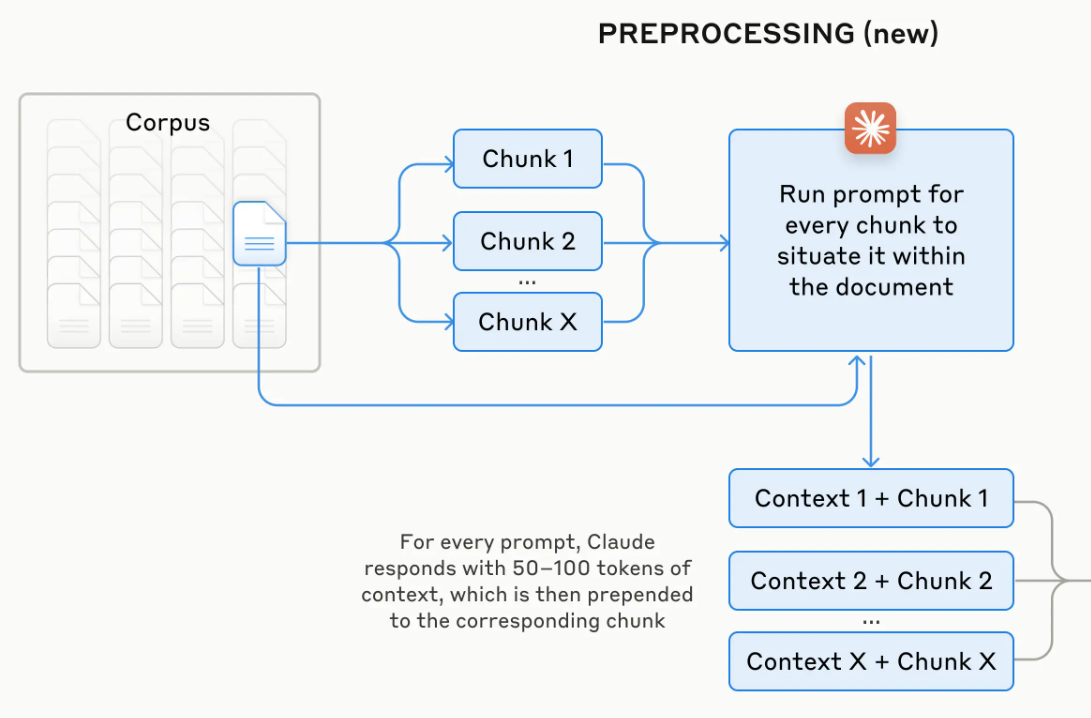
\includegraphics{input/anth_contextual.png}
\caption{Anthropic Contextual Linking \cite{anthropic2024contextualretrieval}}
\label{fig:anth_contextual}
\end{figure}

\subsection{Case Study II: Quiz Generation with Citations}

This case study is motivated by the rise of long-context models (LCs). Developers are encouraged to consider leveraging long-context windows if suitable to application requirements instead of defaulting to a RAGs-based approach given the reasons we have discussed in previous sections where we go over RAGs limitations and trade-offs in relation with LCs.

In this case study, we will build a Quiz generator with citations that explores additional input management techniques particularly useful with long context windows. The implementation includes prompt caching for efficiency and citation tracking to enhance accuracy and verifiability. We will use Gemini\index{Gemini} 1.5 Pro (experimental) as our LLM, which has a context window of 2M tokens.

\subsubsection{Use Case}

Let's assume you are a Harvard student enrolled in GOV 1039 ``The Birth of Modern Democracy'' (see Figure \ref{fig:harvard-class}), you face a daunting reading list for next Tuesday's class on Rights. The readings~\sidenote{If you actually go through the course syllabus you will find that the reading lists are quasi-impossible for a human to complete withing the deadline often including over a thousand pages to read as a weekly assignment.} include foundational documents like the Magna Carta, Declaration of Independence, and US Bill of Rights, each with specific sections to analyze.

\begin{figure}[H]
\centering

\includegraphics{input/harvard.png}
\caption{Harvard's Democratic Theory Class}
\label{fig:harvard-class}
\end{figure}

Instead of trudging through these dense historical texts sequentially, we would like to:
\begin{itemize}
\item Extract key insights and connections between these documents, conversationally.
\item Engage with the material through a quiz format.
\item Add citations to help with verifying answers.
\end{itemize}

\subsubsection{Implementation}

The full implementation is available at Book's Github repository\footnote{\url{https://github.com/souzatharsis/tamingLLMs/tamingllms/notebooks/src/gemini_duo.py}}. Here, we will cover the most relevant parts of the implementation.

\paragraph{Client Class}

First, we will define the \texttt{Client} class which will provide the key interface users will interact with. It has the following summarized interface:

\paragraph{Initialization}
\begin{itemize}
\item \texttt{\_\_init\_\_(knowledge\_base: List[str] = [])}: Initialize with optional list of URLs as knowledge base
\end{itemize}

\textbf{Core Methods}
\begin{itemize}
\item \texttt{add\_knowledge\_base(urls: List[str]) -> None}: Add URLs to the knowledge base
\item \texttt{add(urls: List[str]) -> None}: Extract content from URLs and add to conversation input  
\item \texttt{msg(msg: str = "", add\_citations: bool = False) -> str}: Enables users to send messages to the client
\item \texttt{quiz(add\_citations: bool = True, num\_questions: int = 10) -> str}: Generate a quiz based on full input memory
\end{itemize}

\textbf{Key Attributes:}
\begin{itemize}
\item \texttt{knowledge\_base}: List of URLs providing foundation knowledge
\item \texttt{input}: Current input being studied (short-term memory)
\item \texttt{input\_memory}: Cumulative input + knowledge base (long-term memory)
\item \texttt{response}: Latest response from LLM
\item \texttt{response\_memory}: Cumulative responses (long-term memory)
\item \texttt{urls\_memory}: Cumulative list of processed URLs
\end{itemize}

\paragraph{Corpus-in-Context Prompting\index{Corpus-in-Context Prompting (CiC)}}

The \texttt{add()} method is key since it is used to add content to the client. It takes a list of URLs and extracts the content from each URL using a content extractor (using MarkitDown). The content is then added to the conversation input memory in a way that enables citations using the ``Corpus-in-Context'' (CIC) Prompting \sidecite{lee2024longcontextlanguagemodelssubsume}.

Figure \ref{fig:cic} shows how CIC format is used to enable citations. It inserts a corpus into the prompt. Each candidate citable part (e.g., passage, chapter) in a corpus is assigned a unique identifier (ID) that can be referenced as needed for that task.

\begin{figure}[H]
\centering
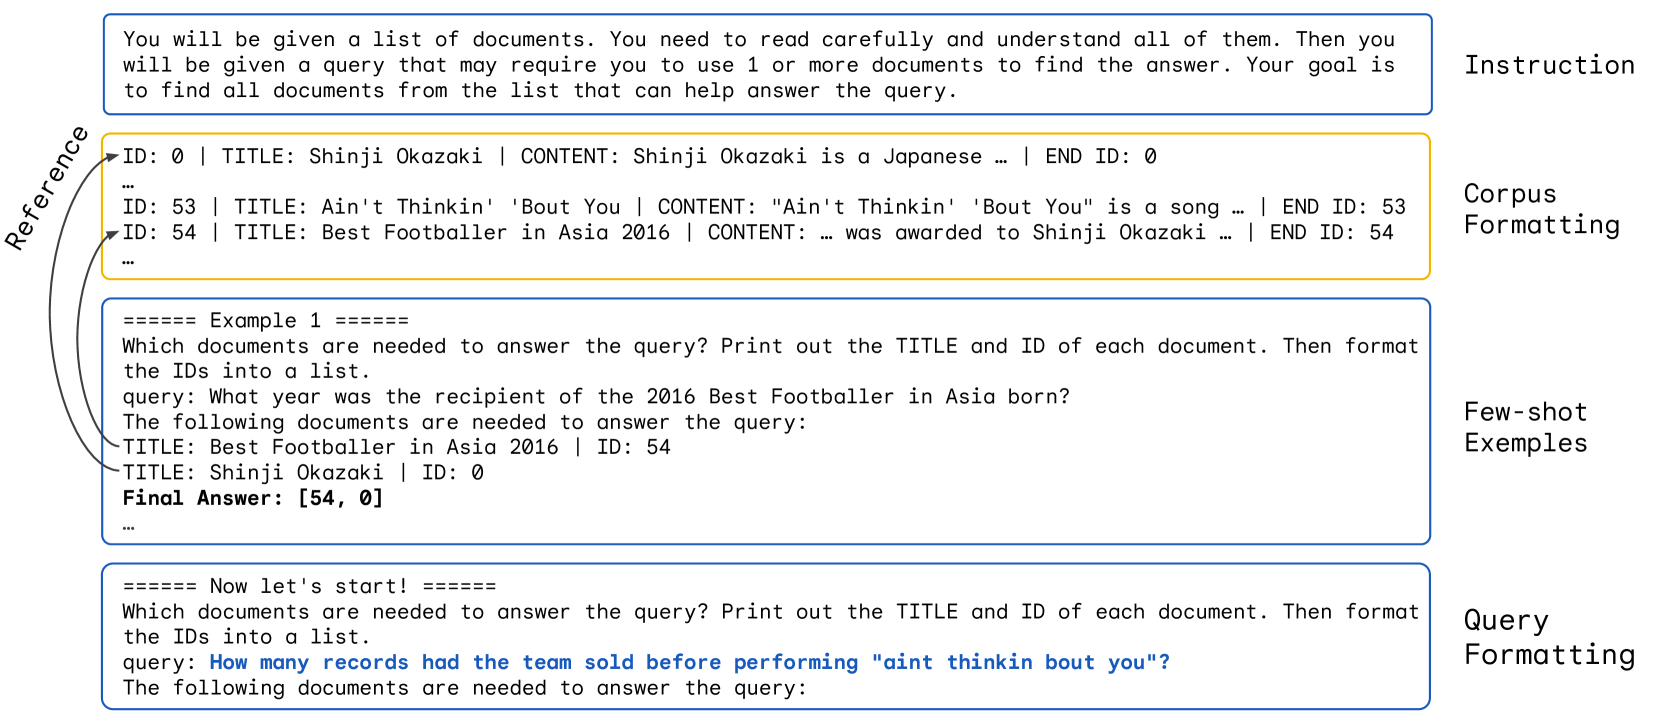
\includegraphics{input/cic.png}
\caption{Example of Corpus-in-Context Prompting for retrieval.}
\label{fig:cic}
\end{figure}

CiC prompting leverages LLM's capacity to follow instructions by carefully annotating the corpus with document IDs. It benefits from a strong, capable models to retrieve over large corpora provided in context.

\begin{minted}{python}
    def add(self, urls: List[str]) -> None:
        self.urls = urls

        # Add new content to input following CIC format to enable citations
        for url in urls:
            self.urls_memory.append(url)
            content = self.extractor.convert(url).text_content
            formatted_content = f"ID: {self.reference_id} | {content} | END ID: {self.reference_id}"
            self.input += formatted_content + "\n" 
            self.reference_id += 1
        
        # Update memory
        self.input_memory = self.input_memory + self.input
\end{minted}

The method \texttt{add\_knowledge\_base()} is a simple wrapper around the \texttt{add()} method. It is used to add URLs to the knowledge base, which are later cached by the LLM model as we will see later.

\begin{minted}{python}
    def add_knowledge_base(self, urls: List[str]) -> None:
        self.add(urls)
\end{minted}

Later, when the user sends a message to the client, the \texttt{msg()} method is used to generate a response while enabling citations. \texttt{self.content\_generator} is an instance of our LLM model, which we will go through next.

\begin{minted}{python}
    def msg(self, msg: str = "", add_citations: bool = False) -> str:
        if add_citations:
            msg = msg + "\n\n For key statements, add Input ID to the response."

        self.response = self.content_generator.generate(
            input_content=self.input,
            user_instructions=msg
        )

        self.response_memory = self.response_memory + self.response.text

        return self.response.text
\end{minted}

\paragraph{Prompt Caching\index{Prompt Caching}}

LLM-based applications often involve repeatedly passing the same input tokens to a model, which can be inefficient and costly. Context caching addresses this by allowing you to cache input tokens after their first use and reference them in subsequent requests. This approach significantly reduces costs~\sidenote{As of January 8th of 2025, cached prompts cost 4x less than uncached for large contexts (over 128k tokens) as per Gemini 1.5 Pro pay-as-you-go pricing~\cite{google2024geminipricing}:
\begin{itemize}
    \item Input Pricing: \$2.50 per 1 million tokens
    \item Output Pricing: \$10.00 per 1 million tokens
    \item Context Caching: \$0.625 per 1 million tokens
\end{itemize}
} compared to repeatedly sending the same token corpus, especially at scale.

In our application, the user might passes a large knowledge base to the client that can be referenced multiple times by smaller user requests. Our \texttt{Client} class is composed of a \texttt{LLMBackend} class that takes the \texttt{input\_memory} containing the entire knowledge base and any additional user added content.

\begin{minted}{python}
self.llm = LLMBackend(input=self.input_memory)
\end{minted}
In our \texttt{LLMBackend} Class, we leverage prompt caching on input tokens and uses them for subsequent requests.

\begin{minted}{python}
class LLMBackend:
    def __init__(self, model_name: str, input: str, cache_ttl: int = 60):
        self.cache = caching.CachedContent.create(
            model=model_name,
            display_name='due_knowledge_base', # used to identify the cache
            system_instruction=(
            self.compose_prompt(input, conversation_config)
        ),
        ttl=datetime.timedelta(minutes=cache_ttl),
    )

    self.model = genai.GenerativeModel.from_cached_content(cached_content=self.cache)
\end{minted}

\textbf{Quiz Generation}

Coming back to our \texttt{Client} class, we implement the \texttt{quiz()} method to generate a quiz based on the full input memory, i.e. the initial knowledge base and any additional user added content.

The \texttt{quiz()} method returns a \texttt{Quiz} instance which behind the scenes caches input tokens. The user later can invoke its \texttt{generate()} method to generate a quiz passing the user instructions in \texttt{msg} parameter, as we will see later.

\begin{minted}{python}
    def quiz(self, add_citations: bool = True, num_questions: int = 10) -> str:
        """
        Returns a quiz instance based on full input memory.
        """
        self.quiz_instance = Quiz(
                         input=self.input_memory,
                         add_citations=add_citations,
                         num_questions=num_questions)
        return self.quiz_instance
\end{minted}

\begin{verbatim}
ROLE:
- You are a Harvard Professor providing a quiz.
INSTRUCTIONS:
- Generate a quiz with {num_questions} questions based on the input.
- The quiz should be multi-choice.
- Answers should be provided at the end of the quiz.
- Questions should have broad coverage of the input including multiple Input IDs.
- Level of difficulty is advanced/hard.
- `{citations}`

STRUCTURE:
- Sequence of questions and alternatives.
- At the end provide the correct answers.
\end{verbatim}
where, \texttt{\{citations\}} instructs the model to add CiC citations to the response if user requests it.

\subsubsection{Example Usage}

\paragraph{Dataset}

First, we will define our knowledge base. 

\begin{itemize}
\item Harvard Class: \href{https://scholar.harvard.edu/files/dlcammack/files/gov_1039_syllabus.pdf}{GOV 1039 Syllabus}
\item Class / Topic: ``Rights''
\item Reading List:
  \begin{enumerate}
  \item The Declaration of Independence of the United States of America
  \item The United States Bill of Rights  
  \item John F. Kennedy's Inaugural Address
  \item Lincoln's Gettysburg Address
  \item The United States Constitution
  \item Give Me Liberty or Give Me Death
  \item The Mayflower Compact
  \item Abraham Lincoln's Second Inaugural Address
  \item Abraham Lincoln's First Inaugural Address
  \end{enumerate}
\end{itemize}

We will take advantage of Project Gutenberg~\sidenote{Project Gutenberg is a volunteer effort to digitize and archive cultural works, to "encourage the creation and distribution of eBooks". It's the oldest digital library, founded in 1971 by Michael S. Hart, who is considered the inventor of the e-book. Project Gutenberg makes it very easy for LLMs since it provides books publicly in text, html and various other formats.} to create our knowledge base.

\begin{minted}{python}
kb = [f"https://www.gutenberg.org/cache/epub/{i}/pg{i}.txt" for i in range(1,9)]
\end{minted}

We will import our module \texttt{gemini\_duo} as \texttt{genai\_duo} and initialize the \texttt{Client} class with our knowledge base.

\begin{minted}{python}
import gemini_duo as genai_duo
from IPython.display import Markdown, display
\end{minted}

\begin{minted}{python}
duo = genai_duo.Client(knowledge_base=kb)
\end{minted}

At this point, we converted each book into markdown using MarkItDown\index{MarkItDown} and cached the content in our LLM model~\sidenote{We can access how many tokens we have cached in our LLM model by looking at the \texttt{usage\_metadata} attribute of the Gemini's model response. At this point, we have cached at total of 38470 tokens.}. Now, we can add references to our knowledge base at anytime by calling the \texttt{add()} method. We add the following references:
\begin{enumerate}
\item The Magna Carta
\item William Shap McKechnie on Magna Carta book
\end{enumerate}

\begin{minted}{python}
study_references = ["https://www.gutenberg.org/cache/epub/10000/pg10000.txt", 
"https://www.gutenberg.org/cache/epub/65363/pg65363.txt"]

duo.add(study_references)
\end{minted}

we can instantiate a \texttt{Quiz} object and generate a quiz based on the full input memory.

\begin{minted}{python}
quiz = duo.quiz(add_citations=True)
display(Markdown(quiz.generate()))
\end{minted}

Figure~\ref{fig:quiz} shows a sample quiz with citations. Marked in yellow are the citations which refer to the input IDs of the resources we added to the model.

\begin{figure*}[h!]
\centering
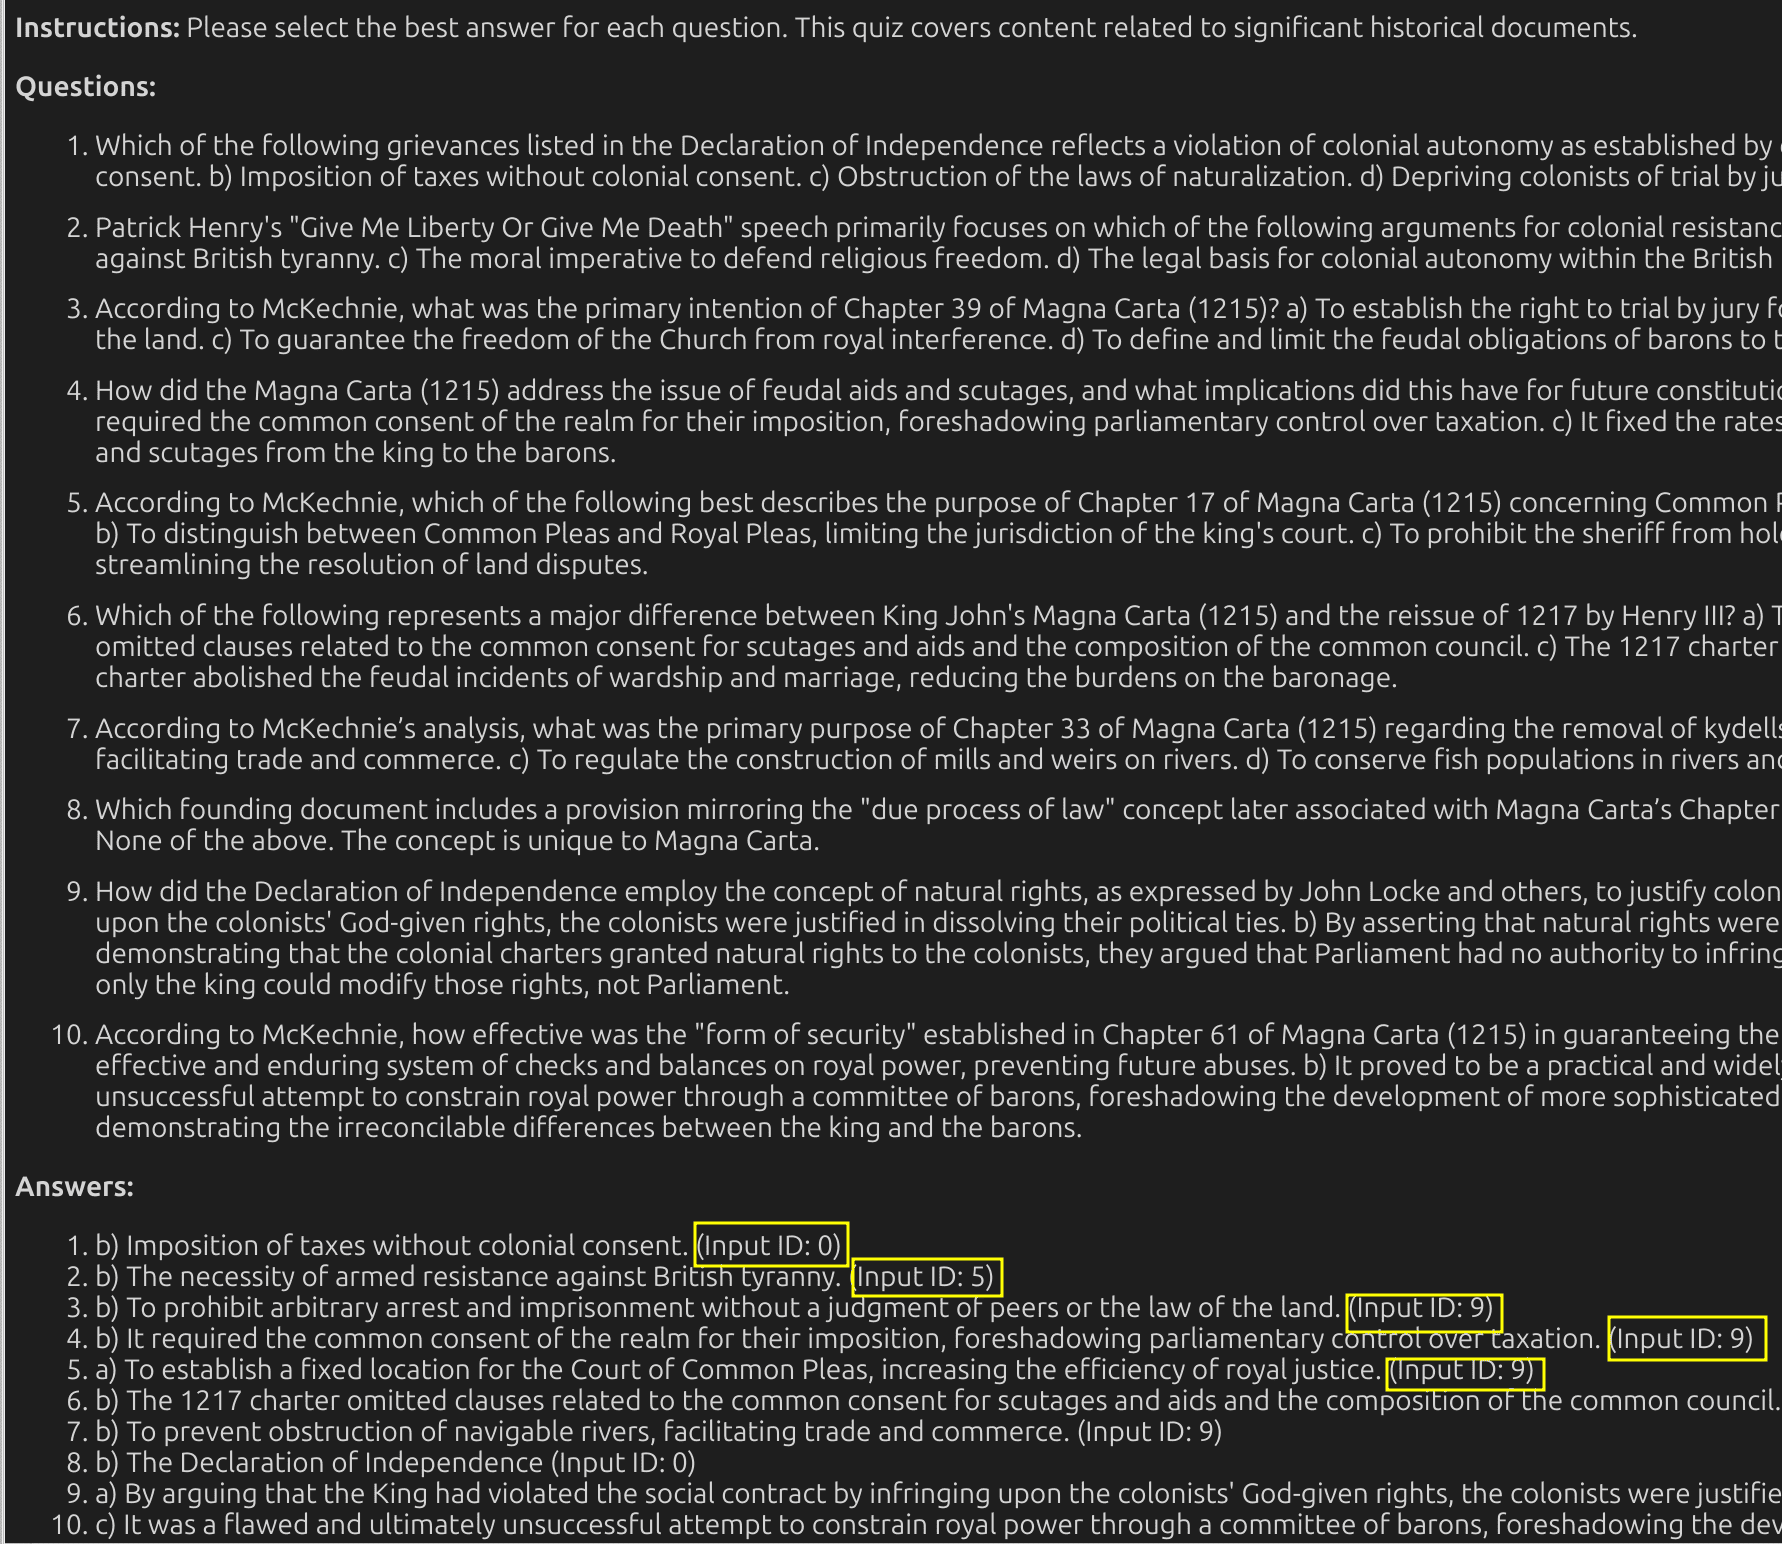
\includegraphics{input/quiz.png}
\caption{Sample Quiz with Citations.}
\label{fig:quiz}
\end{figure*}


\subsubsection{Discussion}

The experiment demonstrated the ability to build a knowledge base from multiple sources while leveraging prompt caching for efficiency and generate quizzes with citations for verifiability. The system successfully ingested content from Project Gutenberg texts, including historical documents like the Magna Carta, and used them to create interactive educational content.

However, several limitations emerged during this process:

\begin{enumerate}
\item Memory Management: The system currently loads all content into memory, which could become problematic with larger knowledge bases. A more scalable approach might involve chunking or streaming the content.

\item Citation Quality: While the system provides citations, they lack specificity - pointing to entire documents rather than specific passages or page numbers. This limits the ability to fact-check or verify specific claims.

\item Content Verification: While citations are provided, the system is not guaranteed to provide factual information. This could lead to potential hallucinations or misinterpretations.
\end{enumerate}

While limitations are present in this simple example, the case study highlights that not always complex systems are needed when working with knowledge bases. Alternative simple strategies should be preferred when possible, particularly if capable, long-context window models are available and fit within the application requirements.

\section{Conclusion}
This chapter has explored critical strategies and techniques for managing input data in LLM applications, focusing on three key areas: data parsing, retrieval augmentation, and practical implementation patterns. We examined how parsing tools such as \texttt{MarkItDown} and \texttt{Docling} can transform diverse data formats into LLM-compatible representations, demonstrating through case studies how parser quality can impact LLM performance. The chapter also investigated retrieval augmentation techniques, particularly RAG systems, showing how they can enhance LLM capabilities by providing access to external knowledge while discussing their future relevance in the context of emerging long-context language models.

Through our case studies, we demonstrated practical approaches to handling common challenges in LLM applications. The Content Chunking with Contextual Linking case study illustrated techniques for managing long-form content generation while maintaining coherence across chunks. The Quiz Generation with Citations case study showcased how long-context windows can be effectively utilized without the need for complex retrieval systems, highlighting the importance of choosing the right approach based on specific application requirements rather than defaulting to more complex solutions.

As the field continues to evolve, the choice between traditional RAG systems and emerging long-context models will likely become increasingly nuanced. While RAGs offer cost-effective solutions for incorporating external knowledge, the rise of long-context models suggests a future where simpler architectures might suffice for many applications. The key insight is that effective input data management requires careful consideration of trade-offs among complexity, cost, and performance, always guided by specific application requirements rather than following a one-size-fits-all approach. Success in building robust LLM applications will depend on understanding these trade-offs and selecting appropriate strategies for each use case.




